\documentclass[a4paper, 10pt, dvipdfmx,draft]{article}

\usepackage[square,sort,comma,numbers]{natbib}

\usepackage{algorithm}      % \begin{algorithm}
\usepackage{algorithmic}    % \begin{algorithmic}
\usepackage{amsmath}        % \begin{align*}
\usepackage{amssymb}        % \mathbb{A}
\usepackage{amsthm}         % \newtheorem
\usepackage{bm,bbm}         % \bm{A}, \bbm{1}
\usepackage{booktabs}       % \toprule, \midrule, \bottomrule
\usepackage{caption}        % \captionsetup
\usepackage{enumitem}       % \begin{enumerate}[label=(\alph*)]
\usepackage{geometry}       % \geometry{margin=1in}
\usepackage{hyperref}       % \href{URL}{text}
\usepackage{ifthen}         % \ifthenelse
\usepackage{mathrsfs}       % \mathscr{A}
\usepackage{mathtools}      % \mathrlap
\usepackage{optidef}        % \begin{mini*}{x}{f(x)}{}{}
\usepackage{physics}        % \qty, \norm, \abs
\usepackage{thm-restate}    % \begin{restatable}{theorem}{thm}
\usepackage{tikz}           % \begin{tikzpicture}
\usepackage{xparse}         % \NewDocumentCommand
% \usepackage{calc}         % \setlength
% \usepackage{cancel}       % \cancel
% \usepackage{parskip}      % \setlength{\parskip}{0.5em}
% \usepackage{csvsimple}    % \csvautotabular
% \usepackage{diagbox}      % \diagbox
% \usepackage{dsfont}       % \mathds{1}
% \usepackage{epsfig}       % \epsfig
% \usepackage{fancybox}     % \ovalbox
\usepackage{float}        % \begin{figure}[H]
% \usepackage{lipsum}       % \lipsum
% \usepackage{listings}     % \begin{lstlisting}
% \usepackage{makecell}     % \makecell{L1\L2}
% \usepackage{multicol}     % \begin{multicols}{2}
% \usepackage{multirow}     % \multirow
% \usepackage{nicematrix}   % \begin{NiceMatrix}
% \usepackage{qcircuit}     % \Qcircuit
% \usepackage{siunitx}      % \SI{1}{\second}
% \usepackage{stfloats}     % \begin{figure*}
\usepackage{subcaption}   % \begin{subfigure}
% \usepackage{subfiles}     % \subfile{file}
% \usepackage{ulem}         % \sout
% \usepackage[hyphens]{url} % \url
% \usepackage{wrapfig}      % \begin{wrapfigure}
% \usepackage[all]{xy}      % \xymatrix
% \usepackage[dvipdfmx]{graphicx}
% \usepackage[square, sort, comma, numbers]{natbib}


\usepackage{cleveref}       % \cref{eq:label}

\geometry{margin=1in}
\hypersetup{colorlinks=true,linkcolor=blue,citecolor=blue,urlcolor=blue}

\definecolor{cA}{HTML}{0072BD}
\definecolor{cB}{HTML}{EDB120}
\definecolor{cC}{HTML}{77AC30}
\definecolor{cD}{HTML}{D95319}

\newcommand{\red}[1]{\textcolor{red}{#1}}
\newcommand{\blue}[1]{\textcolor{blue}{#1}}
\newcommand{\cyan}[1]{\textcolor{cyan}{#1}}
\newcommand{\gray}[1]{\textcolor{gray}{#1}}
\newcommand{\green}[1]{\textcolor{green}{#1}}
\newcommand{\brown}[1]{\textcolor{brown}{#1}}
\newcommand{\black}[1]{\textcolor{black}{#1}}
\newcommand{\st}{\text{ s.t. }}
\newcommand{\Img}[1]{\mathrm{Im}\qty(#1)}
\newcommand{\Ker}[1]{\mathrm{Ker}\qty(#1)}
\newcommand{\Supp}[1]{\mathrm{supp}\qty(#1)}
\newcommand{\Rank}[1]{\mathrm{rank}\qty(#1)}
\newcommand{\floor}[1]{\left\lfloor #1 \right\rfloor}
\newcommand{\ceil}[1]{\left\lceil #1 \right\rceil}
% C++ (https://tex.stackexchange.com/questions/4302/prettiest-way-to-typeset-c-cplusplus)
\newcommand{\Cpp}{C\nolinebreak[4]\hspace{-.05em}\raisebox{.4ex}{\relsize{-3}{\textbf{++}}}}
% https://tex.stackexchange.com/questions/28836/typesetting-the-define-equals-symbol
\newcommand{\defeq}{\coloneqq}
\newcommand{\eqdef}{\eqqcolon}
% https://tex.stackexchange.com/questions/5502/how-to-get-a-mid-binary-relation-that-grows
\newcommand{\relmiddle}[1]{\mathrel{}\middle#1\mathrel{}}

% https://tex.stackexchange.com/questions/564216/newcommand-for-each-letter
\ExplSyntaxOn
\NewDocumentCommand{\definealphabet}{mmmm}{
\int_step_inline:nnn{`#3}{`#4}{
\cs_new_protected:cpx{#1 \char_generate:nn{##1}{11}}{
\exp_not:N #2{\char_generate:nn{##1}{11}}}}}
\ExplSyntaxOff

\definealphabet{bb}{\mathbb}{A}{Z}
\definealphabet{rm}{\mathrm}{A}{Z}
\definealphabet{cal}{\mathcal}{A}{Z}
\definealphabet{frak}{\mathfrak}{a}{z}
% \definealphabet{scr}{\mathscr}{A}{Z}
% \definealphabet{frak}{\mathfrak}{A}{Z}

\newtheorem{theorem}{Theorem}
\newtheorem{proposition}{Proposition}
\newtheorem{lemma}{Lemma}
\newtheorem{definition}{Definition}
\newtheorem{corollary}{Corollary}
\newtheorem{remark}{Remark}
\newtheorem{example}{Example}
\newtheorem{assumption}{Assumption}

% https://qiita.com/rityo_masu/items/efd44bc8f9229e014237
\allowdisplaybreaks[4]

\begin{document}

\title{BackGround Japanese}
\author{M2 48-246226 Hiroki Hamaguchi}
\date{\today}
\maketitle

\section{Newton法}

数値最適化における目的の一つは、目的関数という定量的な評価を最も良くするような決定変数の選択にある。
この目的関数には、設計性能・制御安定性・運用効率・予測誤差など、さまざまな現象やシステムの定量的な質を表すものが挙げられる。
ここで目的関数を$f \colon \bbR^n \to \bbR$と定め、$C^2$級の関数とする。$n$は決定変数の次元数を表す。
そして、次の無制約最適化問題を考える:
\begin{equation}\label{eq:unconstrained-optimization}
    \underset{x \in \bbR^n}{\text{minimize}} \quad f(x).
\end{equation}
本節では、このような問題に対する代表的な二次法の一つである Newton法を扱う。

\subsection{基礎概念}

はじめに、Newton法に関連した、いくつかの重要な基礎概念について述べる。

\subsubsection{凸性と強凸性}

まず、関数$f$が凸であること、および強凸であることは、任意の$x,y \in \bbR^n$に対してそれぞれ次の不等式で定義される:
\begin{align}
    \text{(凸)} \quad
    f(y) & \ge f(x)+\nabla f(x)^\top (y-x),
    \label{eq:convex-def}                                             \\
    \text{($\mu$-強凸)} \quad
    f(y) & \ge f(x)+\nabla f(x)^\top (y-x)+\frac{\mu}{2}\norm{y-x}^2,
    \label{eq:strongly-convex-def}
\end{align}
強凸性は、凸性に加えて目的関数が一様に正の曲率を持つことを表している。
\Cref{fig:convexity_comparison}は、凸関数と強凸関数の具体例を示している。

\begin{figure}[t]
    \centering
    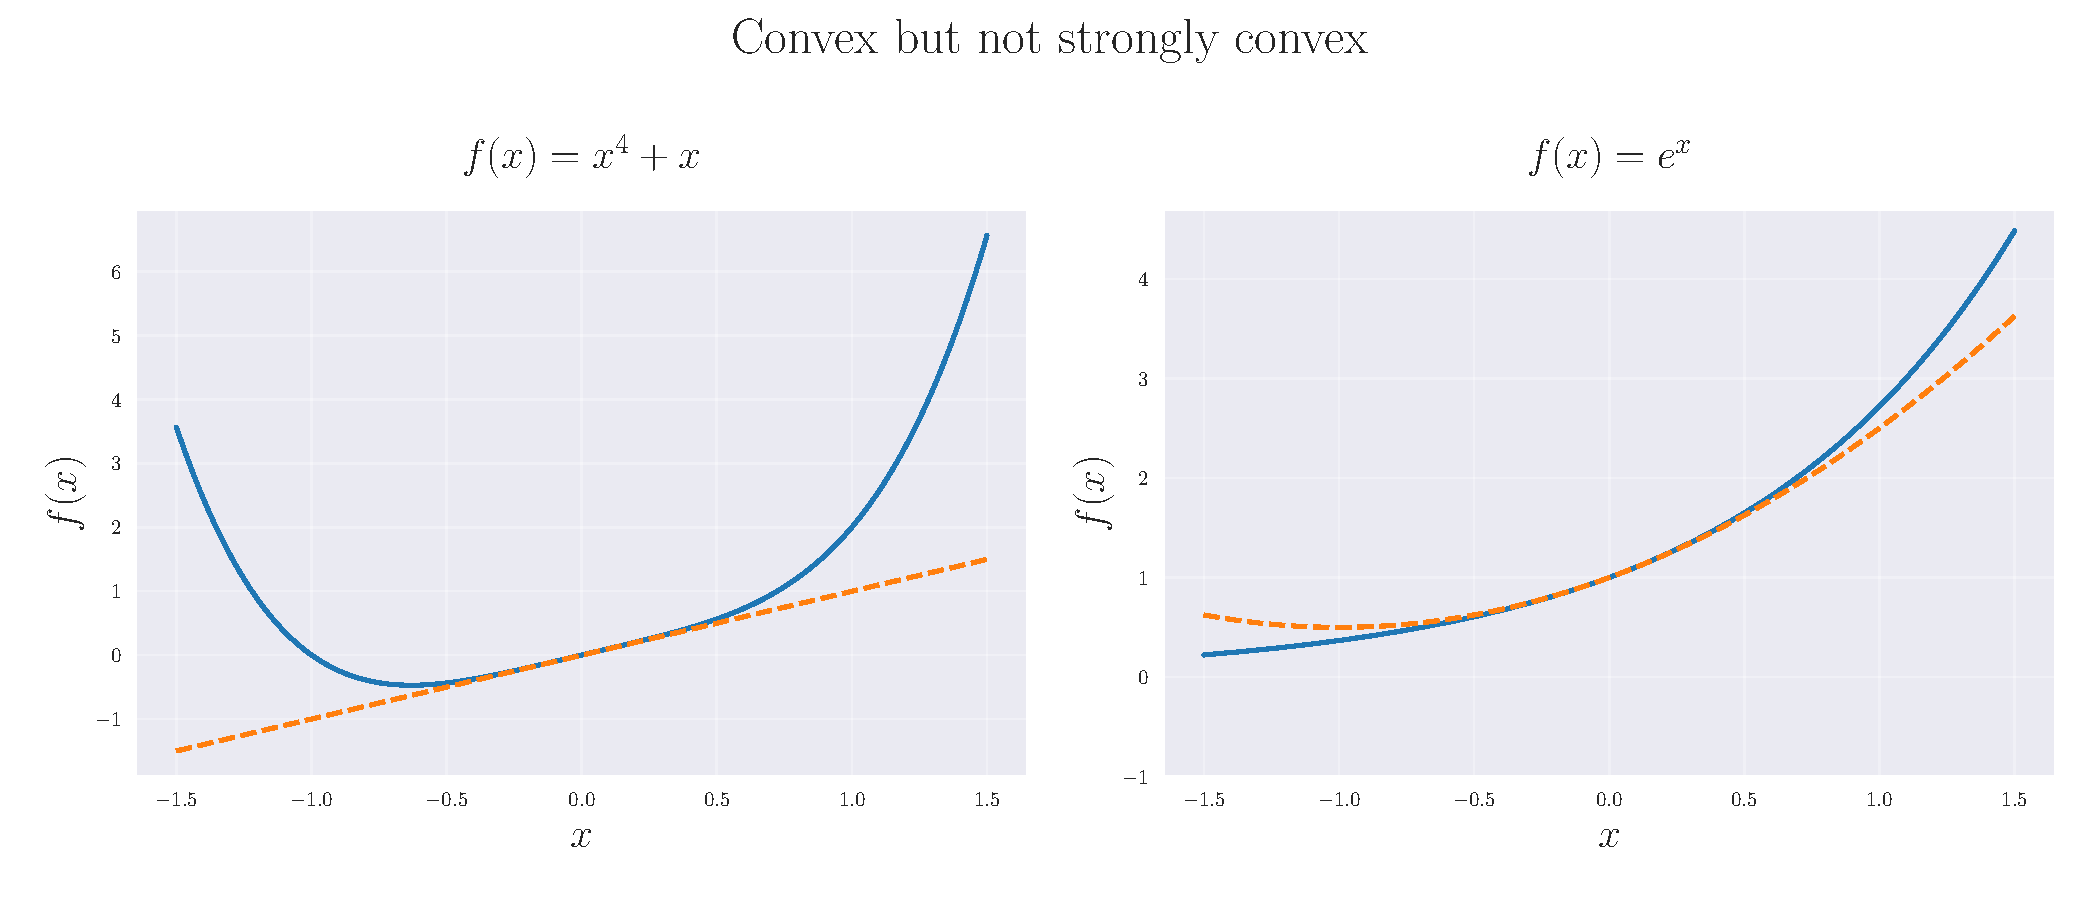
\includegraphics[width=\columnwidth]{../imgs/quasi_newton/convexity_comparison_convex.pdf}
    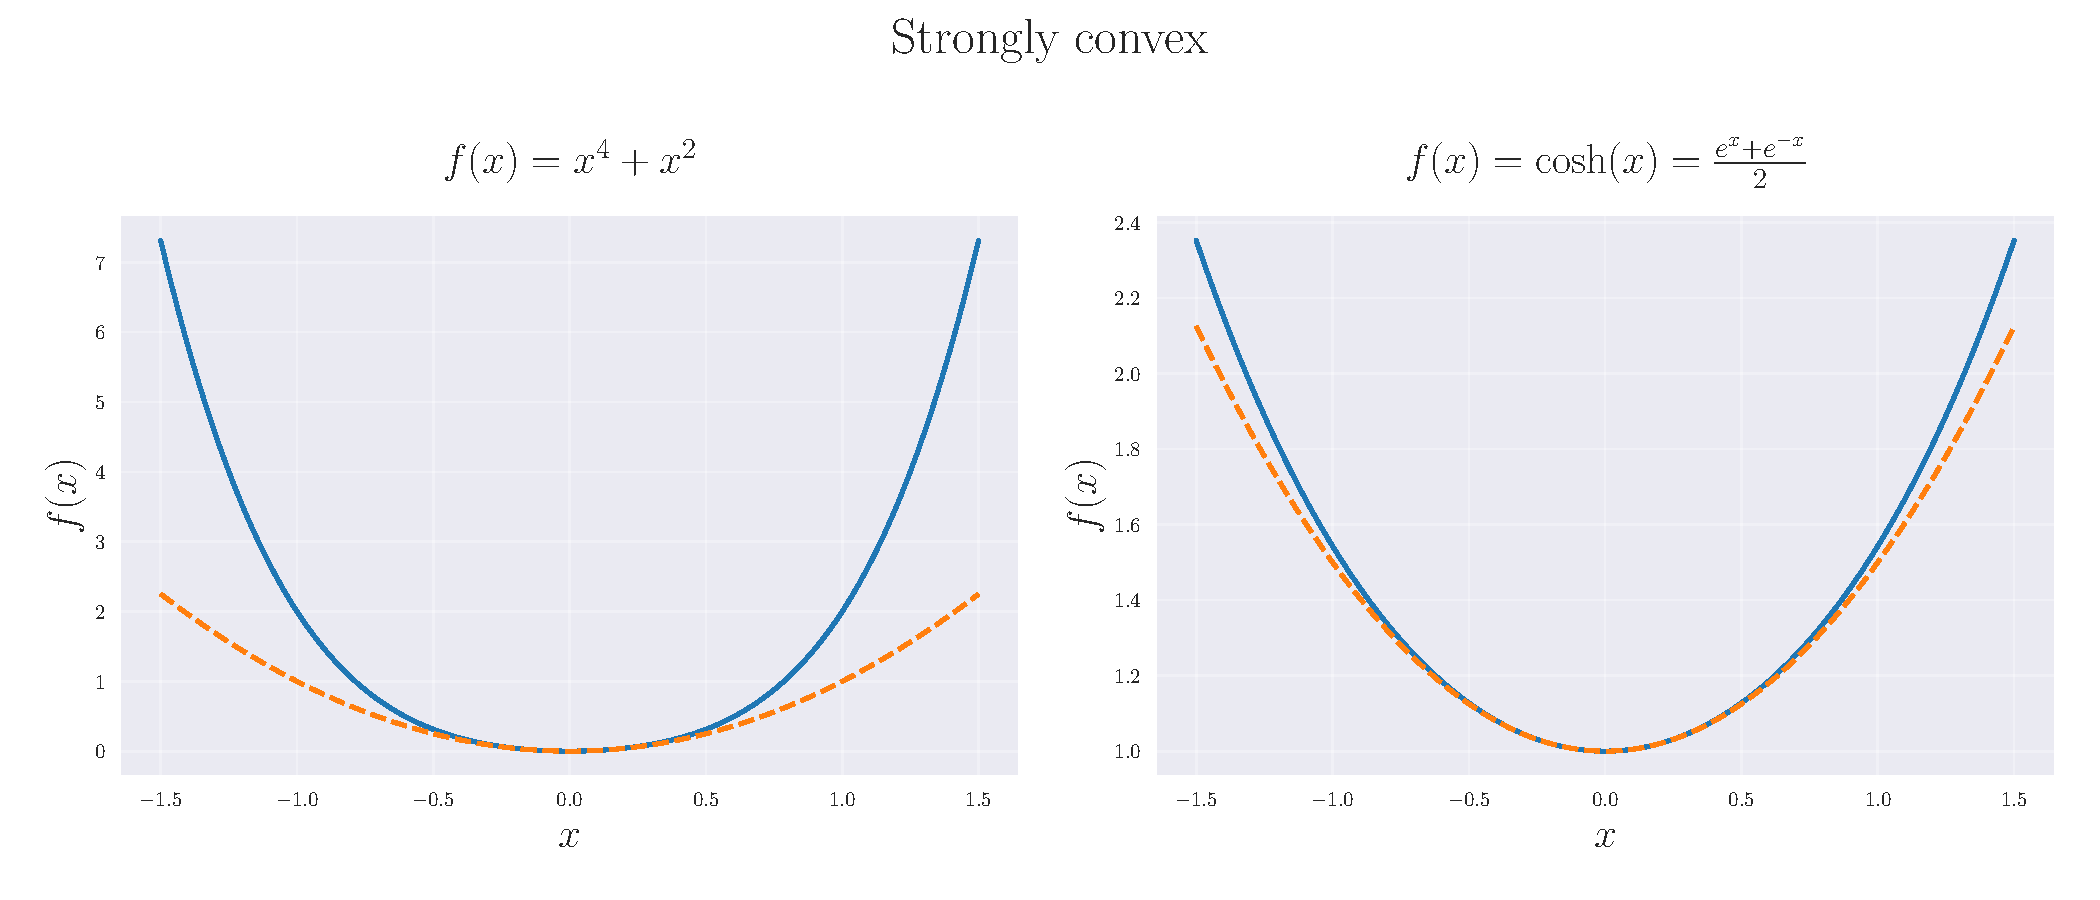
\includegraphics[width=\columnwidth]{../imgs/quasi_newton/convexity_comparison_strongly_convex.pdf}
    \caption{凸関数と強凸関数の比較。点線は$x=0$における二次近似を示す。上二つは凸だが強凸でない関数で、\cref{eq:strongly-convex-def}を満たす$\mu>0$が存在しない。下は強凸な関数で、\cref{eq:strongly-convex-def}を満たす$\mu>0$が存在する。}
    \label{fig:convexity_comparison}
\end{figure}

\subsubsection{ヘッセ行列の正定値性}

次に、凸性や強凸性がヘッセ行列の定値性とどのように関係するかを示す。
行列$A \in \bbR^{n \times n}$が正定値であるとは、任意の非零ベクトル$v \in \bbR^n \setminus \{0\}$に対して$v^\top A v > 0$が成り立つことをいう。これを$A \succ 0$と表記する。半正定値に関しても、$v^\top A v \ge 0$が成り立つ場合を指し、$A \succeq 0$と表記する。
このとき、次の命題が成り立つ。

\begin{proposition}\label{prop:convexity-hessian}
    $f \colon \bbR^n \to \bbR$を$C^2$級関数とする。このとき、
    \begin{itemize}
        \item $f$が凸であることと、任意の$x \in \bbR^n$に対して$\nabla^2 f(x)\succeq0$が成り立つことは同値である。
        \item $f$が$\mu$-強凸であることと、任意の$x \in \bbR^n$に対して$\nabla^2 f(x)\succeq\mu I$が成り立つことは同値である。
    \end{itemize}
\end{proposition}
\begin{proof}
    まず$\mu>0$とし、任意の$x \in \bbR^n$に対して $\nabla^2 f(x)\succeq \mu I$ が成り立つと仮定する。このとき、$f$が$C^2$級であることから、任意の$x,y \in \bbR^n$に対し、
    \begin{equation}\label{eq:taylor-second}
        f(y)
        = f(x)+\nabla f(x)^\top (y-x)
        +\frac{1}{2}(y-x)^\top \nabla^2 f(\xi)(y-x)
    \end{equation}
    を満たす$\xi$が線分$\{x+t(y-x) \mid t\in(0,1)\}$上に存在する。仮定から
    \begin{equation}\label{eq:hessian-strongly-convex}
        (y-x)^\top \nabla^2 f(\xi)(y-x)
        \ge (y-x)^\top \mu I (y-x)
        = \mu\norm{y-x}^2
    \end{equation}
    であるため、\cref{eq:taylor-second}に\cref{eq:hessian-strongly-convex}を代入すると、$\mu$-強凸の定義である\cref{eq:strongly-convex-def}が従う。

    逆に、$f$が$\mu$-強凸であるとき、任意の$x \in \bbR^n$および$v \in \bbR^n$に対して、$y=x \pm tv$とすると、
    \begin{equation}
        f(x \pm tv)\ge f(x) \pm t\nabla f(x)^\top v+\frac{\mu}{2}t^2\norm{v}^2
    \end{equation}
    が成り立つ。
    二つの式を足し合わせて整理すると、
    \begin{equation}\label{eq:strongly-convex-finite-diff}
        f(x+tv)-2f(x)+f(x-tv) \ge \mu t^2 \norm{v}^2
    \end{equation}
    が得られる。
    よって、$\nabla^2 f(x)$の定義に、\cref{eq:strongly-convex-finite-diff}を代入すると、
    \begin{equation}
        v^\top \nabla^2 f(x) v
        = \lim_{t \to 0} \frac{f(x+tv)-2f(x)+f(x-tv)}{t^2}
        \ge \mu\norm{v}^2
    \end{equation}
    が従う。$v \in \bbR^n$は任意であるから、$\nabla^2 f(x)\succeq \mu I$が得られる。

    以上において$\mu=0$とおくことで、\cref{eq:convex-def}に対応する凸性の場合も同様に従う。
    \qed
\end{proof}

なお、\Cref{fig:pd}は、2次関数のヘッセ行列が正定値・不定値・負定値の場合のグラフを示している。正定値性と凸性が対応していることが視覚的に確認できる。

\begin{figure}[t]
    \centering
    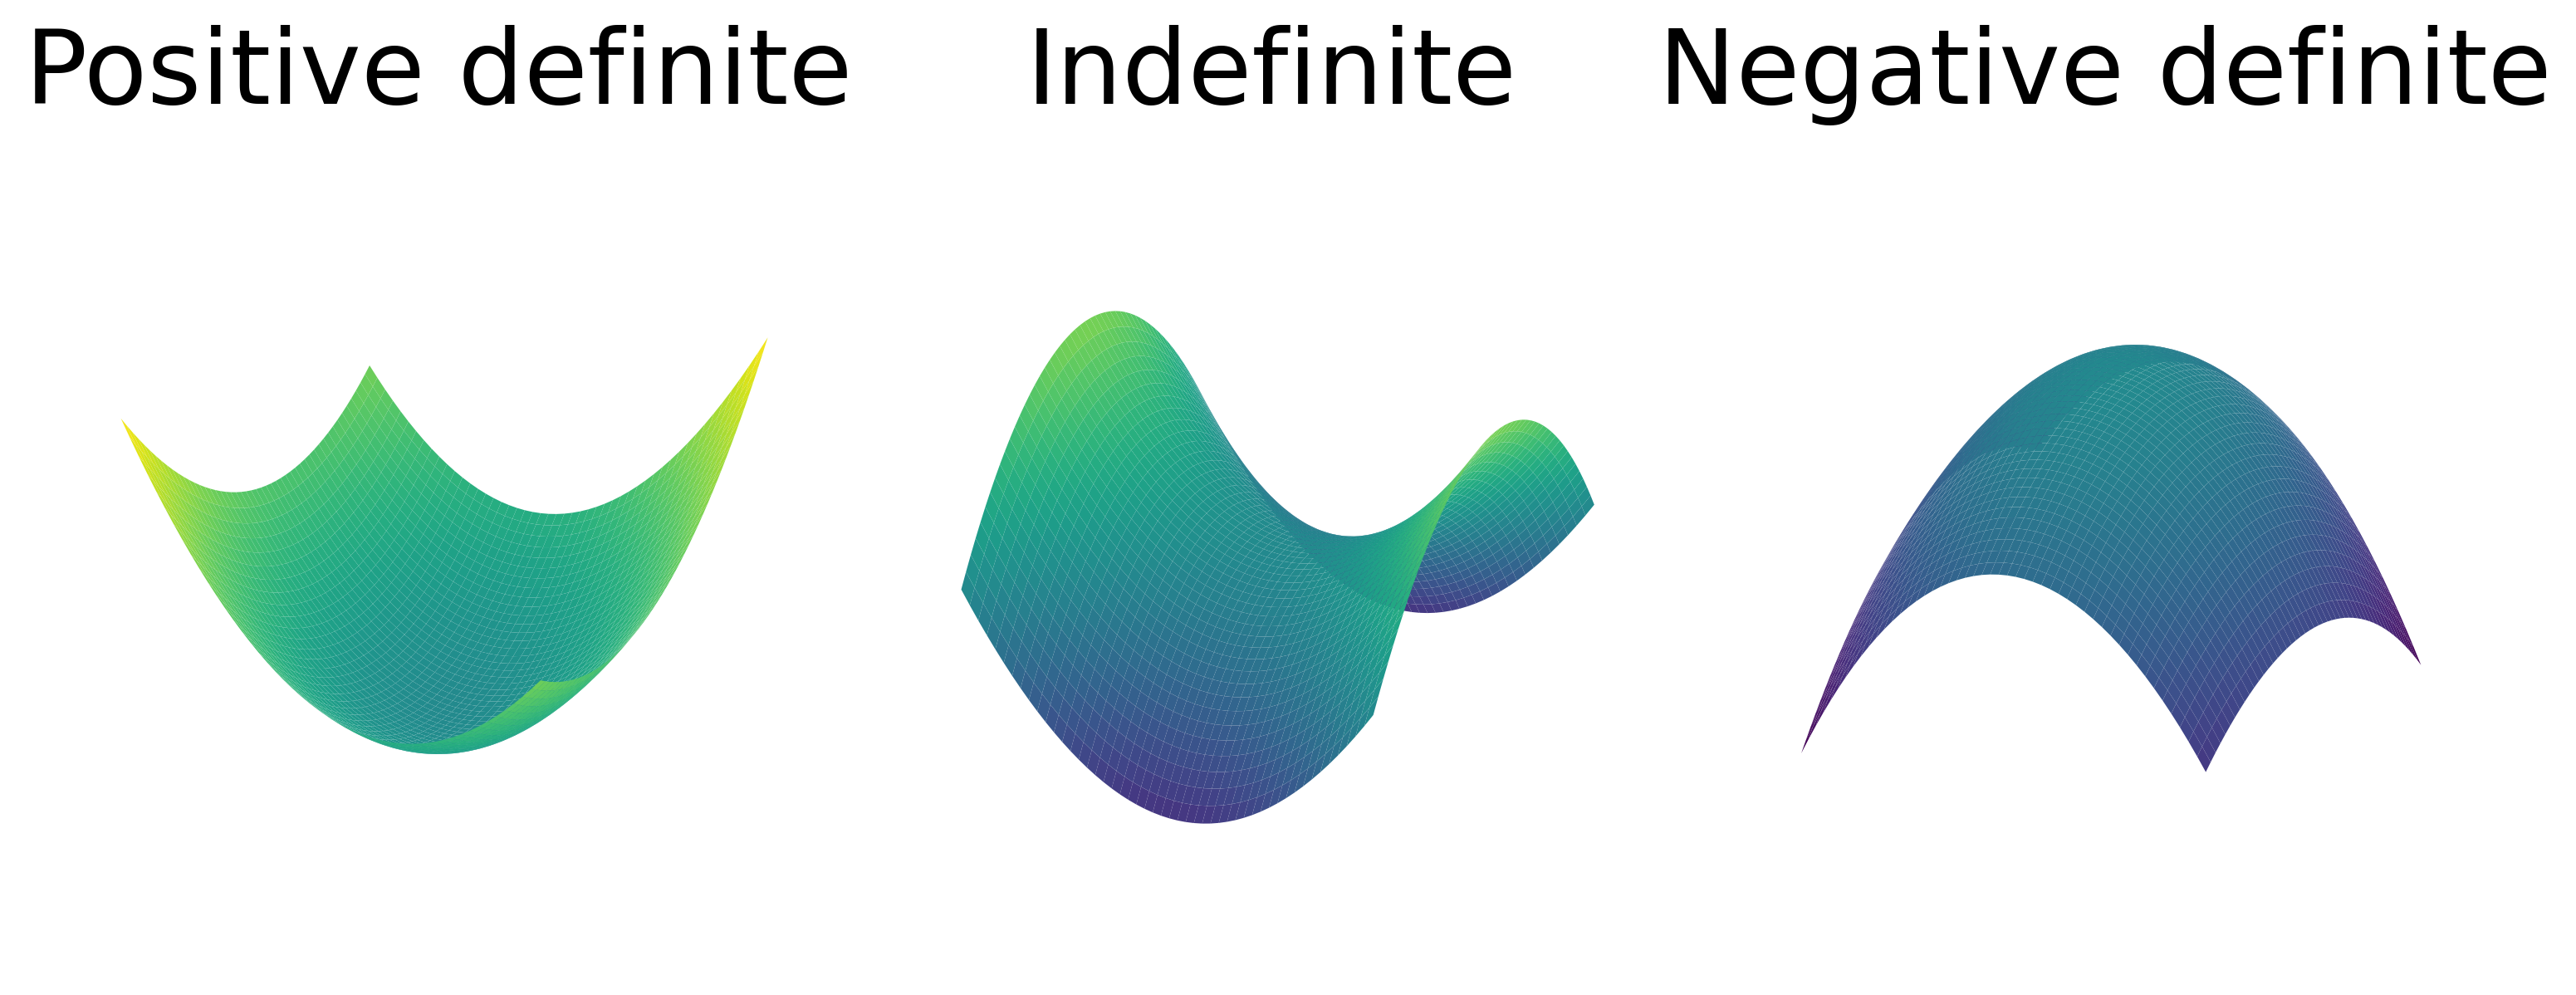
\includegraphics[width=\columnwidth]{../imgs/quasi_newton/pd.png}
    \caption{$x_k$における二次モデル関数のヘッセ行列が (左) 正定値 (中央) 不定値 (右) 不定値 の場合の3次元グラフ}
    \label{fig:pd}
\end{figure}

\subsubsection{$L$-smooth性}

最後に、滑らかさの指標として$L$-smooth性を導入する。$f$が$L$-smoothであるとは、
\begin{equation}
    \norm{\nabla f(x)-\nabla f(y)} \le L\norm{x-y}
\end{equation}
が任意の$x,y$で成り立つことをいう。
$C^2$級の場合、これは$\nabla^2 f(x)\preceq L I$と同値である。

\begin{proposition}\label{prop:smoothness-hessian}
    $f \colon \bbR^n \to \bbR$を$C^2$級関数とする。このとき、$f$が$L$-smoothであることと、任意の$x \in \bbR^n$に対して$\nabla^2 f(x)\preceq L I$が成り立つことは同値である。
\end{proposition}
\begin{proof}
    まず、任意の$x,y \in \bbR^n$に対して
    \begin{equation*}
        \nabla f(y) - \nabla f(x)
        = \int_0^1 \nabla^2 f(x+t(y-x))(y-x) \dd{t}
    \end{equation*}
    が成り立つ。
    ここで、任意の$x \in \bbR^n$に対して$\nabla^2 f(x)\preceq L I$が成り立つと仮定する。このとき、
    \begin{align*}
        \norm{\nabla f(y) - \nabla f(x)}
         & = \norm{\int_0^1 \nabla^2 f(x+t(y-x))(y-x) \dd{t}}   \\
         & \le \int_0^1 \norm{\nabla^2 f(x+t(y-x))(y-x)} \dd{t} \\
         & \le \int_0^1 L\norm{y-x} \dd{t}                      \\
         & = L\norm{y-x}
    \end{align*}
    が従う。

    逆に、$f$が$L$-smoothであるとき、任意の$x \in \bbR^n$および$v \in \bbR^n$に対して、$y=x+tv$とすると、
    \begin{equation*}
        \norm{\nabla f(x+tv)-\nabla f(x)} \le L\norm{tv} = Lt\norm{v}
    \end{equation*}
    が成り立つ。
    両辺を$t$で割り、$t\to0$とすると、
    \begin{equation*}
        v^\top \nabla^2 f(x) v = \lim_{t\to0} \frac{\norm{\nabla f(x+tv)-\nabla f(x)}}{t} \le L\norm{v}^2
    \end{equation*}
    が得られる。$v \in \bbR^n$は任意であるから、$\nabla^2 f(x)\preceq L I$が得られる。
    \qed
\end{proof}

\subsection{Newton法のアルゴリズム}

Newton法は反復法の一種で、初期点 $x_0$ から始めて、逐次的に現在の点を更新し、点列 $\{x_k\}_{k=0}^\infty$ を生成する。この点列が最終的に最適解へと収束することによって、問題\cref{eq:unconstrained-optimization}の解を得ることを目指す。

まず、\cref{eq:unconstrained-optimization}の目的関数が凸であると仮定する。

$k$反復目の点 $x_k$ における勾配 $\nabla f(x_k)$ とヘッセ行列 $\nabla^2 f(x_k)$ を用いると、$x_k$ まわりでの $f$ の二次のテイラー近似モデル $m^*_k \colon \bbR^n \to \bbR$ は次のように与えられる:
\begin{equation}\label{eq:newton-model}
    m^*_{k}(x) \coloneqq f(x_k) + \nabla f(x_k)^\top (x - x_k) + \frac{1}{2} (x - x_k)^\top \nabla^2 f(x_k) (x - x_k).
\end{equation}
このモデルの勾配は
\begin{equation}\label{eq:newton-model-gradient}
    \nabla m^*_k(x) = \nabla f(x_k) + \nabla^2 f(x_k)(x - x_k)
\end{equation}
で与えられる。
二次モデル\cref{eq:newton-model}の最小解はの仮定より $\nabla m^*_k(x) = 0$ を満たす点であるので $\nabla^2 f(x_k)(x - x_k) = -\nabla f(x_k)$ を解くことで得られる:
\begin{equation*}
    \arg\min_{x\in\bbR^n} m^*_{k}(x) = x_k -\nabla^2 f(x_k)^{-1}\nabla f(x_k).
\end{equation*}
単純には、この最小化解を次の反復点として採用すれば良いが、一般にそのような更新では大域的な収束性が保証されないことが知られている。

ヘッセ行列が正定値である場合、関数はその点で局所的に凸であり、Newton法は最適解へ向かう適切な方向を提供する。
一方、ヘッセ行列が負定値または不定値である場合、関数値の減少を保証せず、Newton法は最適解から遠ざかる方向を示すことがある。不定値の場合は関数値が減少することもあるが、その分鞍点に陥るリスクも高まる。
したがって、Newton法の適用に際しては、ヘッセ行列の正定値性を確認することが重要である。

そこで、直線探索型のNewton法では、更新方向 $d_k \coloneqq -\nabla^2 f(x_k)^{-1}\nabla f(x_k)$ に対し、ステップ幅 $\alpha_k>0$ をラインサーチによって決定した、次のような更新式が採用される:
\begin{equation*}
    x_{k+1} \gets x_k + \alpha_k d_k.
\end{equation*}
(尤も、$f$が非凸関数の場合には、$d_k$が上昇方向となる可能性がある為、全ての連続関数に対して大域的収束性が保証される訳ではない。修正Newton法(modified Newton method)\citep[Sec. 3.4]{nocedal1999numerical}はその対処法の一つと知られるが、本節では扱わない。)
これがNewton法の基本形である。

Newton法は、局所的には二次的な収束速度を示し、一般に高速な収束を実現することで知られる。
しかしながら、ヘッセ行列 $\nabla^2 f(x_k) \in \bbR^{n \times n}$ の計算や線形方程式 $\nabla^2 f(x_k) d_k = -\nabla f(x_k)$ の求解は、時間計算量 $\order{n^3}$を要する。その為、大規模問題では準Newton法(quasi-Newton method)などの他の最適化手法も用いられるが、ここではその前提として、Newton法を概説していく。

\subsection{求根アルゴリズムとしてのNewton法との比較}

数値数学および最適化理論においては、互いに関連しつつも異なる二つの Newton法がしばしば登場する。
それは「求根アルゴリズムとしてのNewton法」と「最適化におけるNewton法」である。

\subsubsection{求根アルゴリズムとしてのNewton法}

単にNewton法(あるいは Newton--Raphson法) と言う場合、$g\colon \bbR \to \bbR$ という微分可能なスカラー関数に対して、$g(x) = 0$ を解く求根アルゴリズムを指すことがある。この手法は本節の主題ではないが、より基本的かつ広く知られているようである。

初期値 $x_0$ から出発すると、その反復式は次のように与えられる:
\begin{equation*}
    x_{k+1} = x_k - \frac{g(x_k)}{g'(x_k)}.
\end{equation*}
幾何的には、$x_k$ 近傍での $g$ のグラフをその接線で近似し、その接線が $x$ 軸と交わる点を次の近似解とする操作に対応する。
詳細は \href{https://en.wikipedia.org/wiki/Newton%27s_method}{Wikipedia: Newton's method} を参照されたい。

\subsubsection{最適化におけるNewton法}

最適化の文脈でNewton法という場合、$f\colon \mathbb R^{n} \to\bbR$という二階微分可能な関数に対して、その局所最小点、あるいはその必要条件として停留点 $\nabla f(x) = 0$ を求めるアルゴリズムを指すことが多い。こちらが本節の主たる関心対象である。

各反復においてヘッセ行列 $\nabla^2 f(x)$ が正定値であると仮定していたことを再掲する。
最適化における Newton法とは、求根アルゴリズムの枠組みを勾配 $\nabla f(x)$ に適用したものである:
\begin{equation*}
    x_{k+1} = x_k - \nabla^2 f(x_k)^{-1} \nabla f(x_k).
\end{equation*}
スカラー関数の場合には $x_{k+1}=x_k - f'(x_k) / f''(x_k)$ に帰着する。
詳細は \href{https://en.wikipedia.org/wiki/Newton%27s_method_in_optimization}{Wikipedia: Newton's method in optimization} を参照されたい。

\subsubsection{二つの定式化の関係}

\begin{figure}[H]
    \centering
    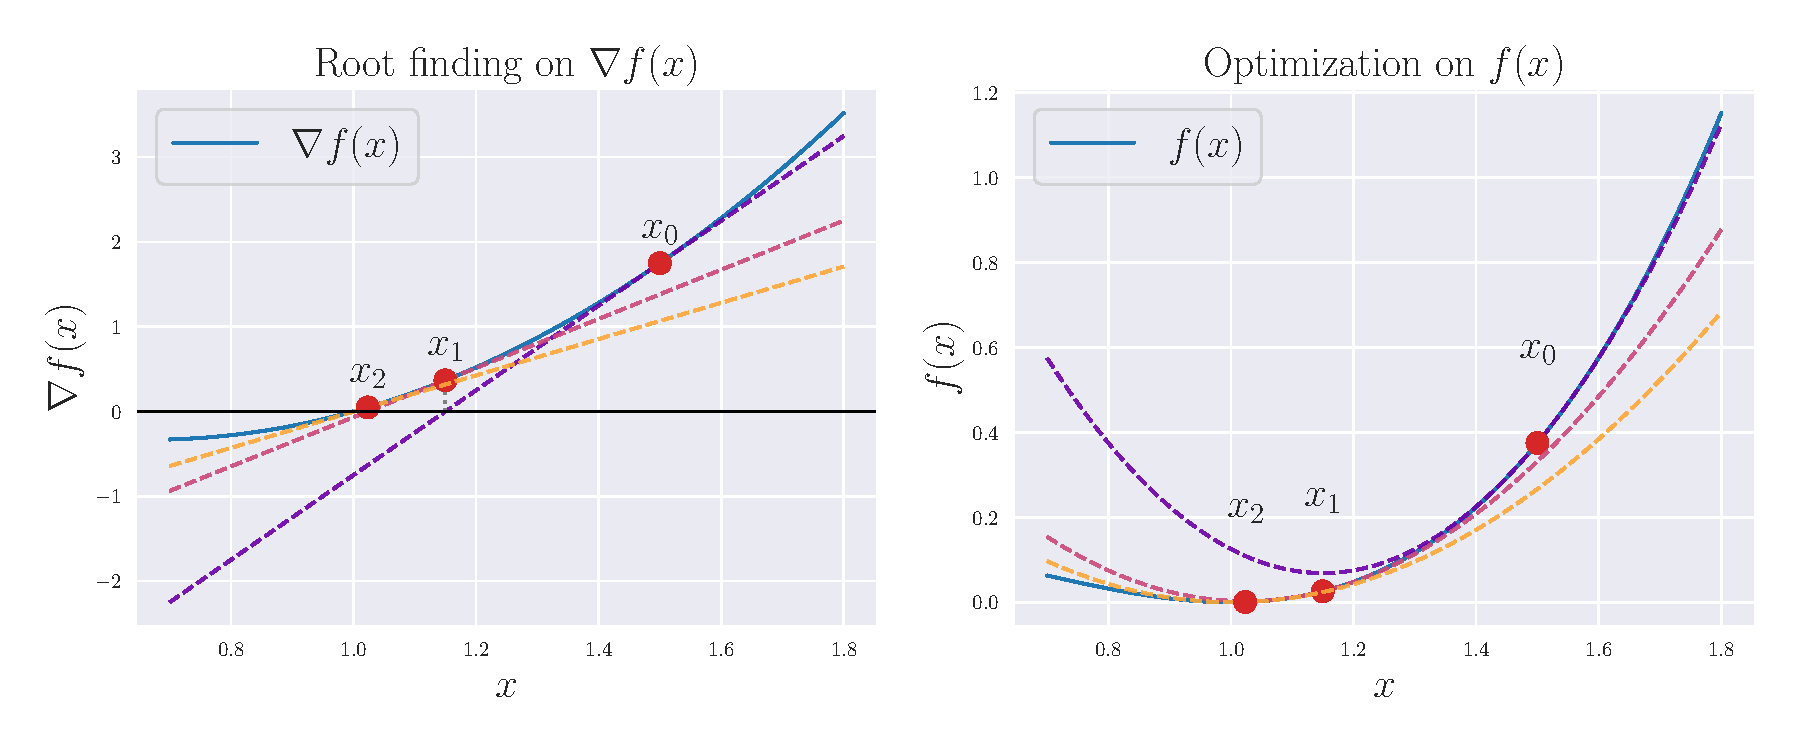
\includegraphics[width=\columnwidth]{../imgs/quasi_newton/newton_raphson.pdf}
    \caption{勾配 $\nabla f(x)=3 x^2 - 4 x + 1$ に対する求根と関数 $f(x)=x^3 - 2 x^2 + x$ に対する最適化}
    \label{fig:newton_raphson}
\end{figure}

具体例を通して、二つの定式化の等価性を確認しよう。
\Cref{fig:newton_raphson}は、単純な三次関数 $f(x)$ を用いて、これら二つの定式化の関係を図示している。
左側は $g(x) = \nabla f(x)$ に対する求根、右側は $f(x)$ に対する最適化を示している。

求根アルゴリズムとしての定式化では、$\nabla f(x) = 3x^2 - 4x + 1$ をその接線、すなわち
\begin{equation*}
    \nabla m^*_k(x) = \nabla f(x_k) + \nabla^2 f(x_k)(x - x_k)
\end{equation*}
で近似し、その線形モデルの根を $x_{k+1}$ として選んでいる。

一方、最適化アルゴリズムとしてのの定式化では、$f(x) = x^3 - 2x^2 + x$ を二次のテイラー展開
\begin{equation*}
    m^*_k(x) = f(x_k) + \nabla f(x_k)(x - x_k) + \frac{1}{2}\nabla^2 f(x_k)(x - x_k)^2
\end{equation*}
で近似し、この二次モデルの最小化解を $x_{k+1}$ とする。

したがって、正定値性の仮定のもとで、両者が本質的に等価な操作をしていることは、局所解の性質から明らかで、その対応関係も確認できる。

以下では、最適化の定式化のみを考察する。

\subsection{収束性に関する性質}
\label{sec:newton-local-convergence}

本節の最後に、Newton法の標準的な局所収束定理を示す。
ここでは簡潔さのために簡略化した形で述べる(完全な定理については \cite[Thm.~3.5]{nocedal1999numerical} を参照) 。

\begin{theorem}[{\cite[Thm.~3.5]{nocedal1999numerical}}]
    \label{thm:newton-quadratic}
    ヘッセ行列 $\nabla^2 f(x)$ が解 $x^*$ の近傍で Lipschitz 連続であり、さらに十分な二次最適性条件(すなわち $\nabla f(x^*)=0$ かつ $\nabla^2 f(x^*)$ が正定値) を満たしているとする。
    すべての $k$ に対して $\alpha_k=1$ とし、$x_0$ が十分に $x^*$ に近い場合、
    勾配ノルム列 $\{\|\nabla f(x_k)\|\}$ は二次収束する。
\end{theorem}
\begin{proof}
    Newton ステップの定義と最適性条件 $\nabla f(x^*)=0$ から次が成り立つ:
    \begin{align*}
        x_{k+1} - x^*
         & = x_k - x^* - \qty(\nabla^2 f(x_k))^{-1}\nabla f(x_k)                                          \\
         & = \qty(\nabla^2 f(x_k))^{-1} \qty(\nabla^2 f(x_k)(x_k-x^*)-\qty(\nabla f(x_k)-\nabla f(x^*))).
    \end{align*}
    Taylor の定理と三角不等式より、
    \begin{align*}
                & \norm{\nabla^2 f(x_k)(x_k-x^*)-\qty(\nabla f(x_k)-\nabla f(x^*))}                          \\
        =   {}  & \norm{\nabla^2 f(x_k)(x_k-x^*)-\qty(\int_0^1 \nabla^2 f(x_k+t(x^*-x_k)) (x_k - x^*)\dd t)} \\
        \leq {} & \int_0^1 \norm{\nabla^2 f(x_k)-\nabla^2 f(x_k+t(x^*-x_k))}\norm{x_k-x^*}\dd t.
    \end{align*}
    $\nabla^2 f$ が Lipschitz 定数 $L$ で連続ならば、被積分関数は $Lt\norm{x_k-x^*}$ で抑えられ、積分すると次を得る:
    \begin{equation*}
        \norm{\nabla^2 f(x_k)(x_k-x^*)-\qty(\nabla f(x_k)-\nabla f(x^*))}
        \le \frac{1}{2}L\|x_k-x^*\|^2.
    \end{equation*}

    $\nabla^2 f(x^*)$ が正則であるため、ある半径 $r>0$ が存在し、$\|x_k-x^*\|\le r$ を満たす全ての $x_k$ について
    $\norm{\qty(\nabla^2 f(x_k))^{-1}}\le 2\norm{\qty(\nabla^2 f(x^*))^{-1}}$ が成り立つ。
    以上を組み合わせると
    \begin{equation*}
        \|x_{k+1} - x^*\|
        \le L\norm{\qty(\nabla^2 f(x^*))^{-1}} \,\|x_k-x^*\|^2.
    \end{equation*}
    $\widetilde L  \defeq  L\norm{\qty(\nabla^2 f(x^*))^{-1}}$ とおき、$\|x_0-x^*\|\le \min\{r,1/(2\widetilde L)\}$ となるように初期点を選べば、帰納的議論により $\{x_k\}$ は近傍内に留まり、$x^*$ へ収束する。
    上式の誤差評価から、$\{x_k\}$ の二次収束性が得られる。

    勾配ノルムの二次収束を示すために、$x_{k+1}-x_k=-\qty(\nabla^2 f(x_k))^{-1}\nabla f(x_k)$ および
    $\nabla f(x_k)+\nabla^2 f(x_k)\qty(x_{k+1}-x_k)=0$ を用いると、
    \begin{align*}
        \norm{\nabla f(x_{k+1})}
         & = \norm{\nabla f(x_{k+1})-\nabla f(x_k)-\nabla^2 f(x_k)\qty(x_{k+1}-x_k)}                 \\
         & \le \int_0^1 \norm{\nabla^2 f(x_k+t (x_{k+1}-x_k))-\nabla^2 f(x_k)}\,\|x_{k+1}-x_k\|\dd t \\
         & \le \frac{1}{2}L\|x_{k+1}-x_k\|^2                                                         \\
         & \le \frac{1}{2}L\norm{\qty(\nabla^2 f(x_k))^{-1}}^2\|\nabla f(x_k)\|^2                    \\
         & \le 2L\norm{\qty(\nabla^2 f(x^*))^{-1}}^2\|\nabla f(x_k)\|^2,
    \end{align*}
    よって $\|\nabla f(x_k)\|$ は二次的にゼロへ収束する。
\end{proof}

\subsection{大域的収束性のための要素}

先述の通り、Newton法ではヘッセ行列の正定値性と、line search によるステップサイズの選択が重要な役割を果たす。
これらは、Newton法の大域的収束性を保証するために必ずしも必要ではないが、一般には広くこれらの要素が採用されている。
\Cref{tab:newton_convergence}に、これらの要素と収束性の関係をまとめる。

\begin{table}[htbp]
    \centering
    \caption{Newton法におけるステップ選択と収束性の概要}
    \label{tab:newton_convergence}
    \begin{tabular}{lll}
        \toprule
        ステップ選択                  & 凸性 & 収束性 / 備考                                                \\
        \midrule
        $\alpha_k=1$            & 強凸 & 局所二次収束（\cref{sec:newton-local-convergence}）             \\
        $\alpha_k=1$            & 強凸 & 大域収束しない例あり（\cref{sec:newton-fullstep}）                  \\
        Line search             & 強凸 & 大域収束する（適切な条件下）（\cref{todo}）                             \\
        Line search             & 非凸 & 大域収束しない例あり（\cref{sec:newton-pd}）                        \\
        Line search + 修正Newton法 & 非凸 & 適切な仮定の下で停留点へ大域収束 \citep[Thm.~3.8]{nocedal1999numerical} \\
        \bottomrule
    \end{tabular}
\end{table}

本小節では、何故これらの要素が必要とされるかについて述べる。

\subsubsection{フルステップの問題点}
\label{sec:newton-fullstep}

Newton法では、各反復においてステップサイズ $\alpha_k=1$ を採用してしまうと、問題が生じる場合がある。ここではその例を示すと共に、その解決策としての line search の必要性について述べる。

\paragraph{Newton法が発散する例}

次のような関数を考えると、Newton法は初期条件によって発散することがある。
\begin{align*}
    f(x)   & = \sqrt{1 + x^2},            \\
    f'(x)  & = \frac{x}{\sqrt{1 + x^2}},  \\
    f''(x) & = \frac{1}{(1 + x^2)^{3/2}}.
\end{align*}
初期点の絶対値が1より大きい場合、\cref{fig:newton_failure_sqrt_function}に示すように、
Newton法を適用すると発散する。

\begin{figure}[H]
    \centering
    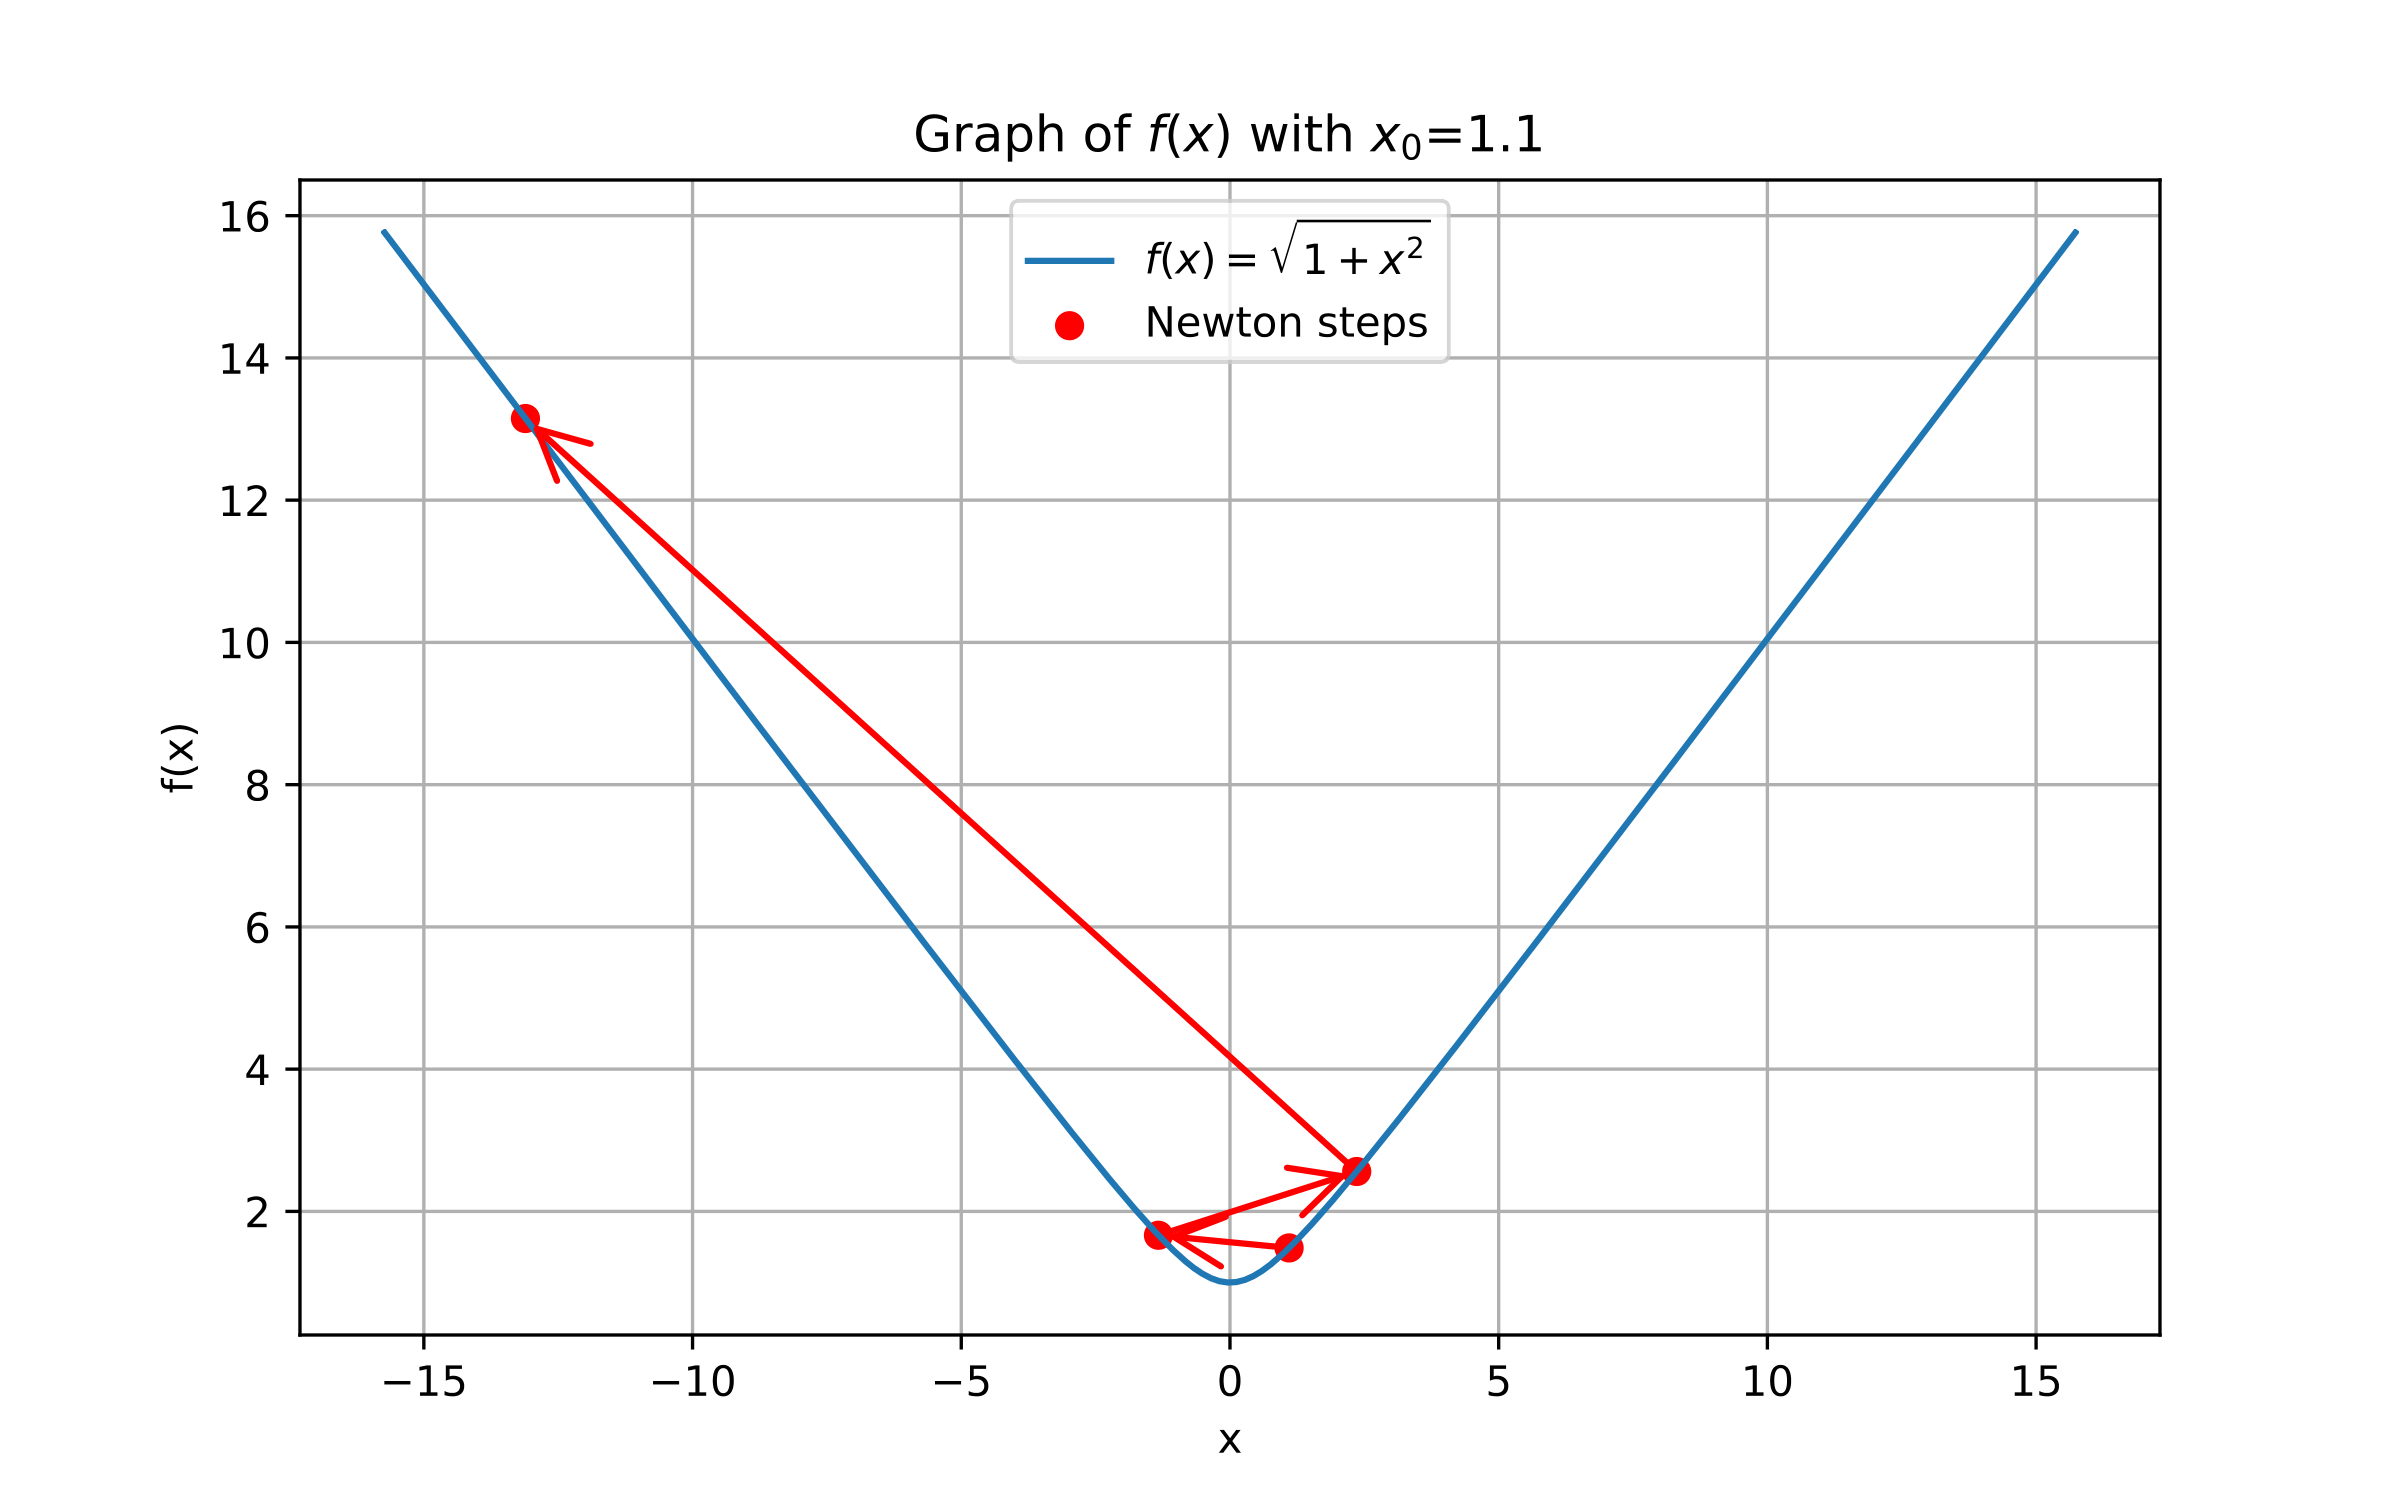
\includegraphics[width=0.6\columnwidth]{../imgs/quasi_newton/newton_failure_sqrt_function_1.1.png}
    \caption{初期点 $x_0=1.1$ の場合 Newton法が発散する例}
    \label{fig:newton_failure_sqrt_function}
\end{figure}

\paragraph{強凸関数に対するNewton法の振動例}

先ほどのNewton法が発散する例では、目的関数が強凸でなく、必ずしも良い性質を持った目的関数とは言えない。
しかし、強凸性というかなり良い性質を持った関数に対しても、Newton法が収束しない例が存在し、その一つがDoikov (2021) の Example 1.4.3 (\href{https://dial.uclouvain.be/pr/boreal/object/boreal:260515}{Doikov, New second-order and tensor methods in convex optimization}) である。

この例では、$\mu>0$ に対して次の関数を考える:
\begin{align*}
    f(x)     & = \log(1 + e^x) - \frac{x}{2} + \frac{\mu x^2}{2}, \\
    f'(x)    & = \frac{e^x}{1+e^x} - \frac{1}{2} + \mu x,         \\
    f''(x)   & = \frac{e^x}{(1+e^x)^2} + \mu,                     \\
    f'''(x)  & = \frac{e^x(1 - e^x)}{(1+e^x)^3},                  \\
    f''''(x) & = \frac{e^x(1 - 4e^x + e^{2x})}{(1+e^x)^4}.
\end{align*}

この関数は以下の性質を持つ:
\begin{enumerate}[nosep,label=\textbullet]
    \item $\mu$-強凸である。
    \item $\max_x |f''(x)| = \frac{1}{4} + \mu$($e^x=1$ のとき)。したがって $\nabla f$ は $L$-smooth($L=\frac{1}{4}+\mu$)。
    \item $\max_x |f'''(x)| = \frac{1}{6\sqrt{3}}$($e^x=2-\sqrt{3}$ のとき)。したがって $\nabla^2 f$ は $M$-Lipschitz($M=\frac{1}{6\sqrt{3}}$)。
\end{enumerate}

しかしながら、$\mu$ に対して初期点 $x_0$ が十分大きい場合、\cref{fig:newton_failure_strongly_convex_function}に示すように、
Newton法を適用すると振動する。

\begin{figure}[H]
    \begin{minipage}{0.5\columnwidth}
        \centering
        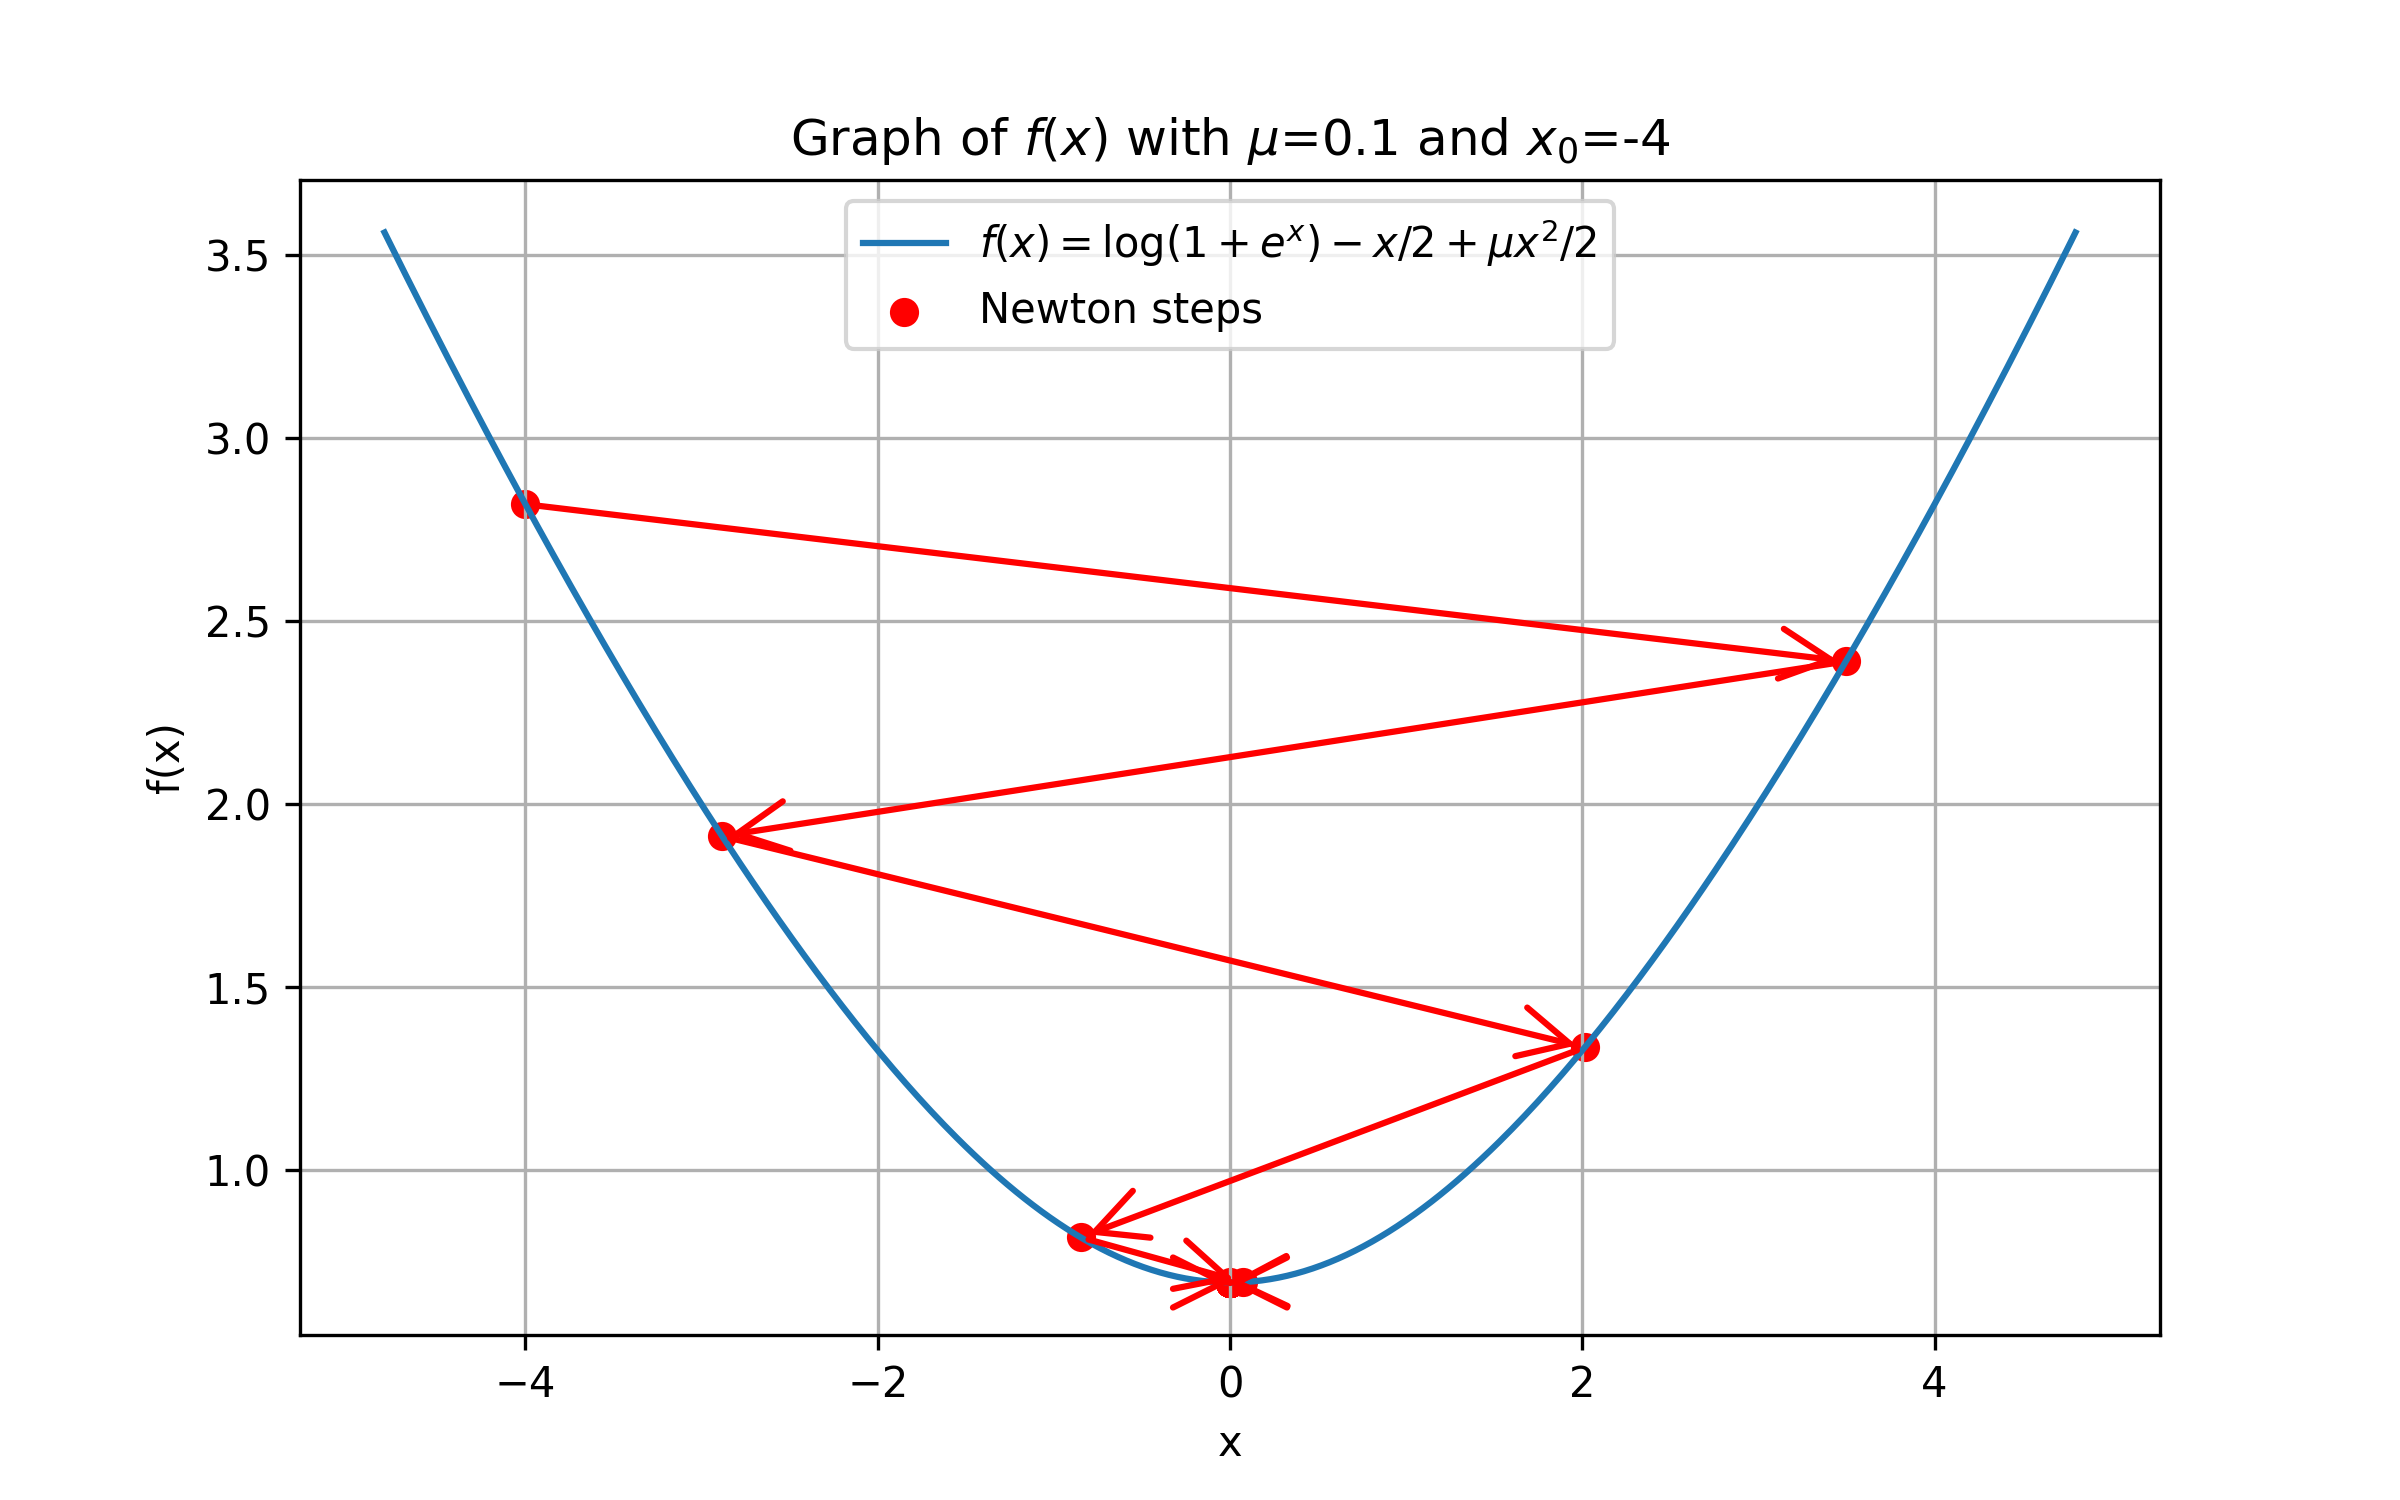
\includegraphics[width=\columnwidth]{../imgs/quasi_newton/newton_failure_strongly_convex_function_0.1_-4.png}
    \end{minipage}%
    \begin{minipage}{0.5\columnwidth}
        \centering
        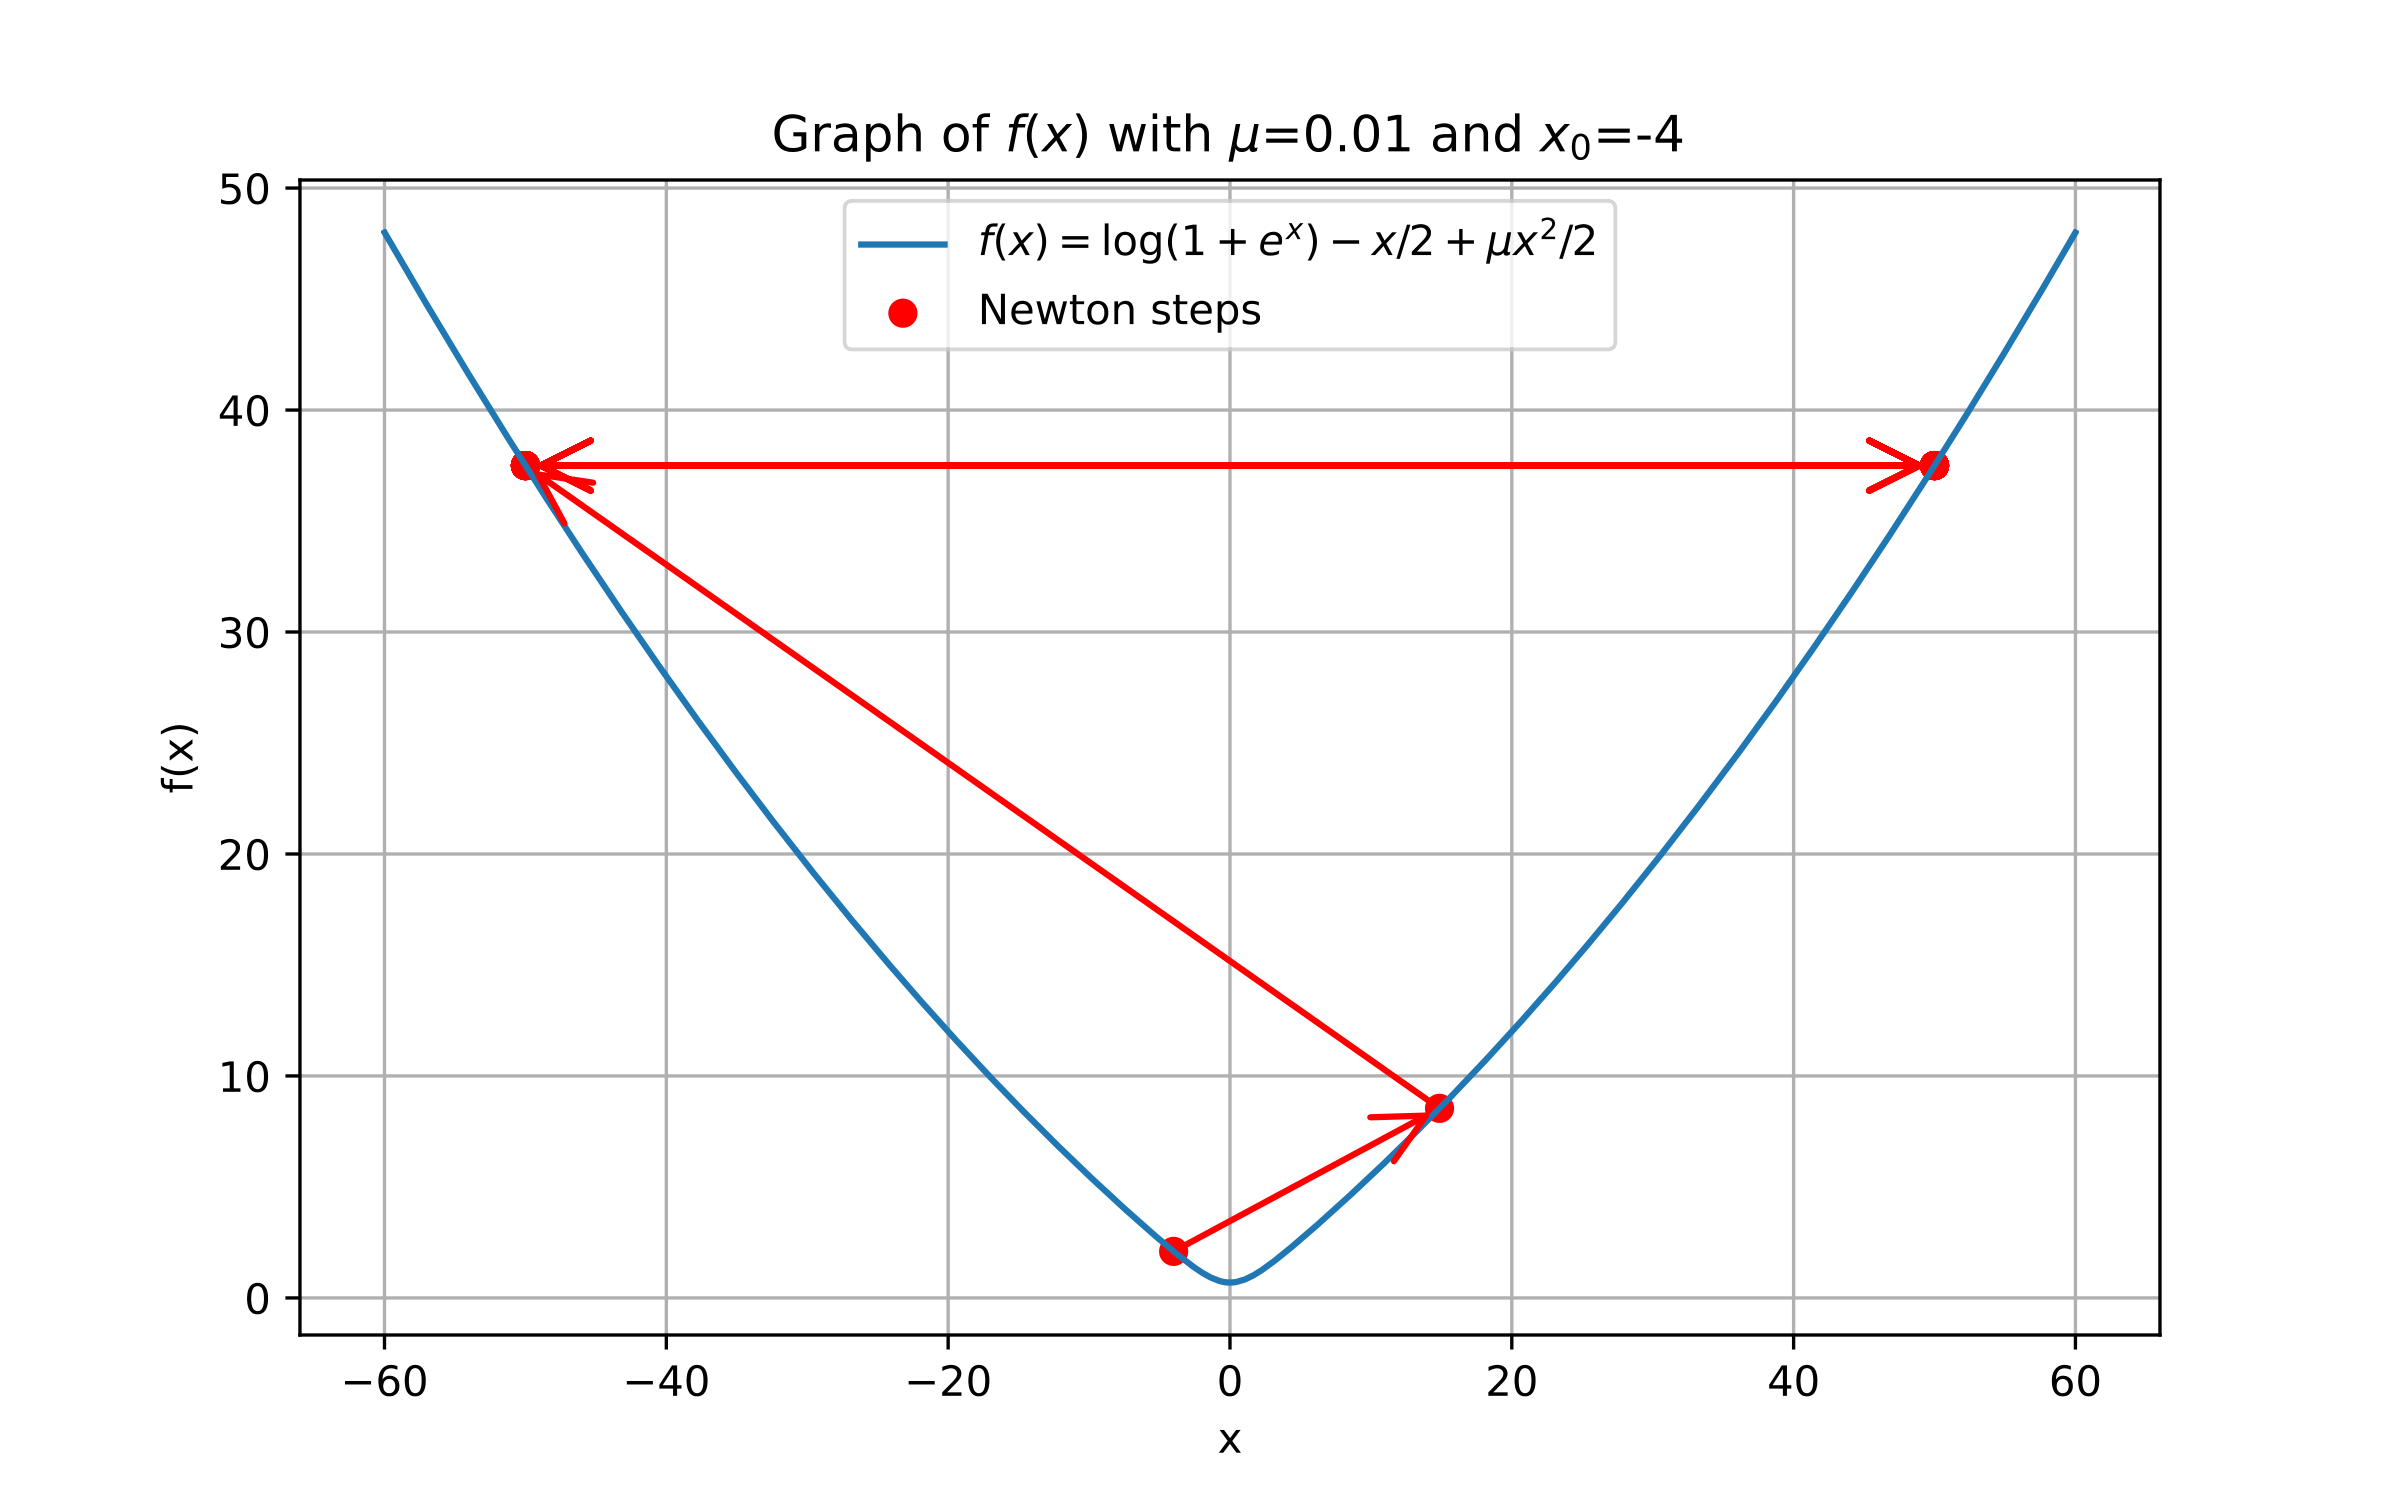
\includegraphics[width=\columnwidth]{../imgs/quasi_newton/newton_failure_strongly_convex_function_0.01_-4.png}
    \end{minipage}
    \caption{(左) 初期点 $x_0=-4, \ \mu=0.1$ の場合 Newton法は収束する例 (右) 初期点 $x_0=-4, \ \mu=0.01$ の場合 Newton法が振動する例}
    \label{fig:newton_failure_strongly_convex_function}
\end{figure}

\paragraph{Line Search の必要性}

以上のような問題を回避するために、Newton法では line search によってステップサイズ $\alpha_k$ を適切に選択することが一般的である。
このように、line searchを導入したNewton法は、一般に修正Newton法(modified Newton method)とも呼ばれ、大域的収束性を持つことが知られている。

\section{準Newton法}

\begin{figure}[htbp]
    \centering
    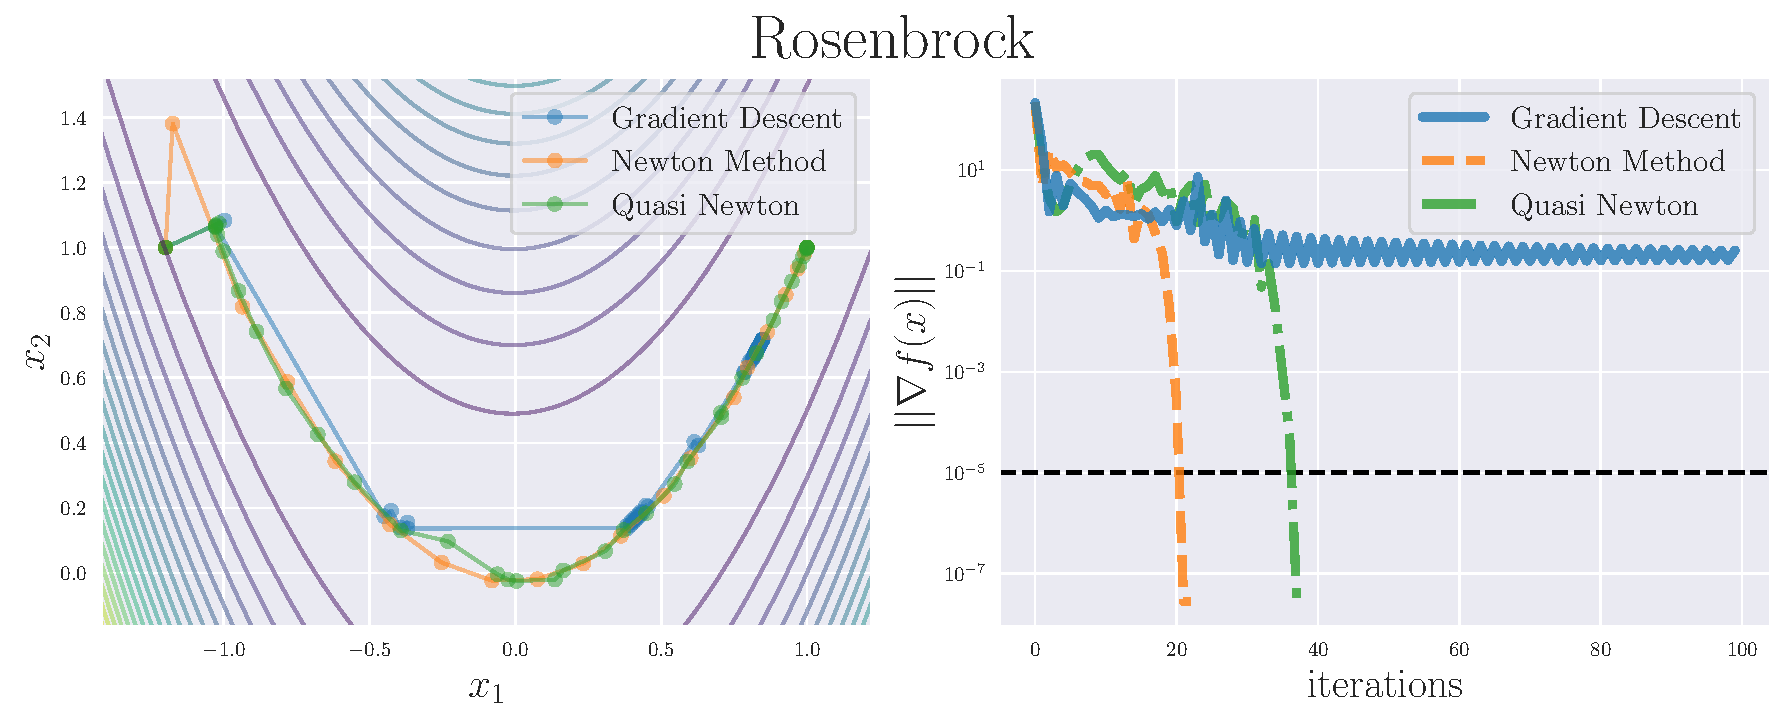
\includegraphics[width=\columnwidth]{../imgs/quasi_newton/newton_vs_qs_vs_gd.pdf}
    \caption{Newton法、準Newton法、勾配降下法の比較}
    \label{fig:newton_vs_qs_vs_gd}
\end{figure}

本節では、準Newton法 (quasi-Newton method) について述べる。準Newton法は、Newton法をベースとしながら、その最大の問題点であったヘッセ行列の計算コストを削減することを目的とした一次法である。つまり、真のヘッセ行列 $\nabla^2 f(x_k)$ の代わりに、その近似行列 $B_k$ を用いることで、計算コストを抑えつつも高速な収束を実現する手法である。

\Cref{fig:newton_vs_qs_vs_gd}に、Newton法、準Newton法、勾配降下法の比較を示した。勾配降下法とは、単に勾配の逆方向に更新を行う手法であり、イテレーション毎の計算コストは最も低いが、収束が遅い。
Newton法は反復回数の点では最も高速であるが、1ステップあたりの計算コストが最も高い。準Newton法はこれら二つの特性の中間に位置し、バランスを取る。特に、iteration数ではなく計算時間で比較した場合、準Newton法は最良の性能を示すことが多い。

直線探索型の準Newton法は、最適解 $x^*$ に収束する一連の近似 $\{ x_k \}_{k=0}^{\infty}$ を次のように生成する:
\begin{equation*}
    x_{k+1} = x_k - \alpha_k B_k^{-1} \nabla f(x_k)
    = x_k - \alpha_k H_k \nabla f(x_k)
\end{equation*}
ここで、$\alpha_k > 0$ は直線探索(line search) によって決定されるステップ幅、$B_k$ は点 $x_k$ におけるヘッセ行列 $\nabla^2 f(x_k)$ の近似、$H_k \coloneqq B_k^{-1}$ はその逆行列である。

\begin{figure}[htbp]
    \begin{minipage}{0.33\columnwidth}
        \centering
        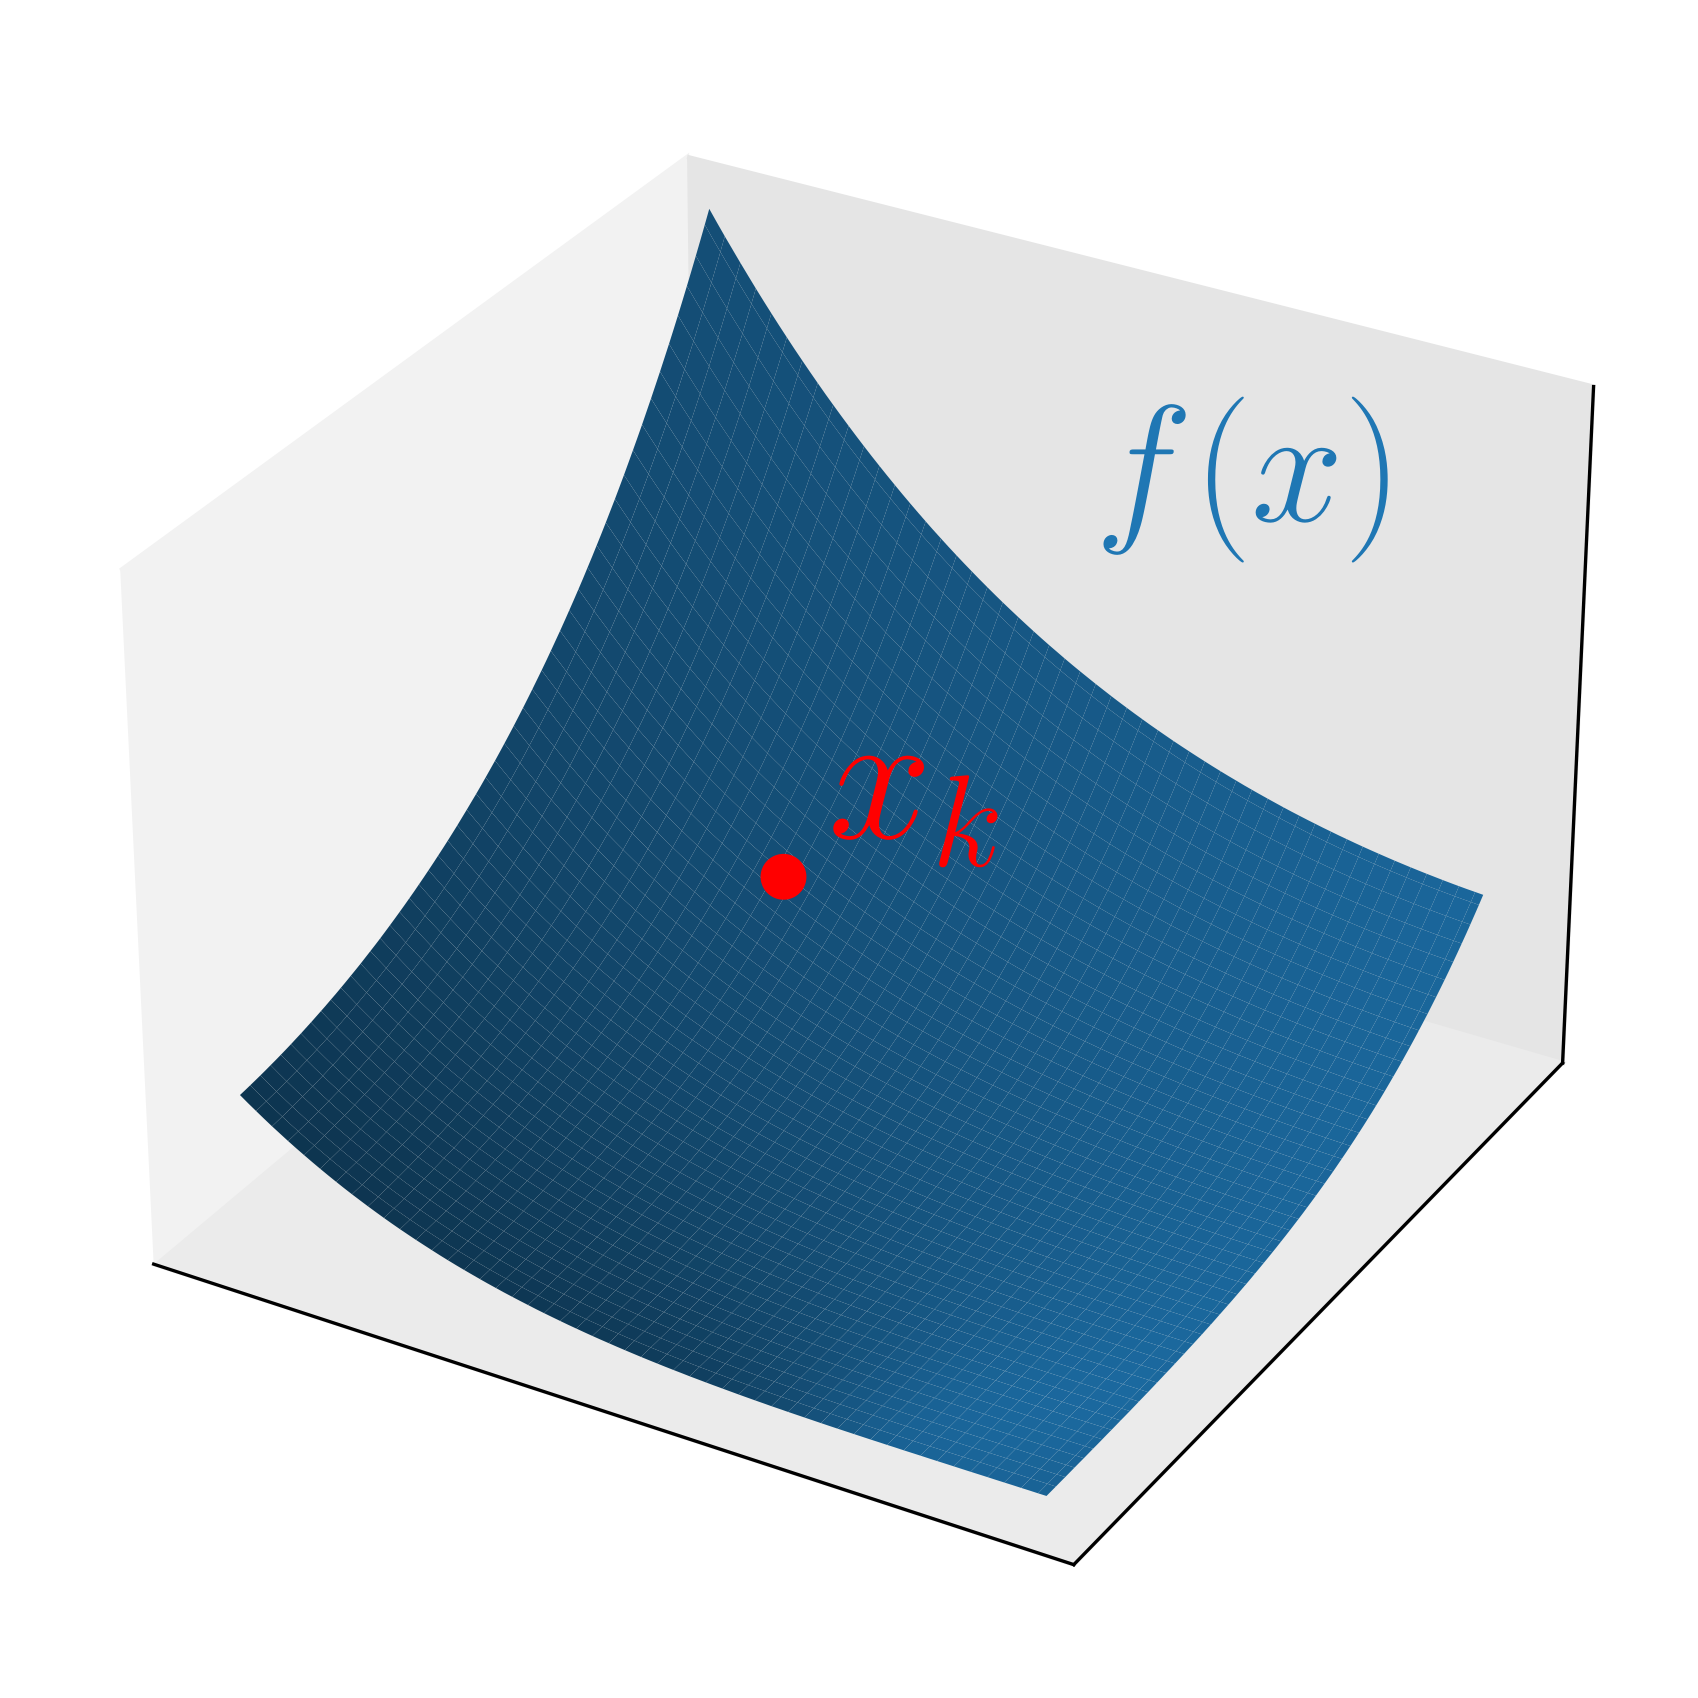
\includegraphics[width=\columnwidth]{../imgs/quasi_newton/quasi_newton_1.png}
    \end{minipage}%
    \begin{minipage}{0.33\columnwidth}
        \centering
        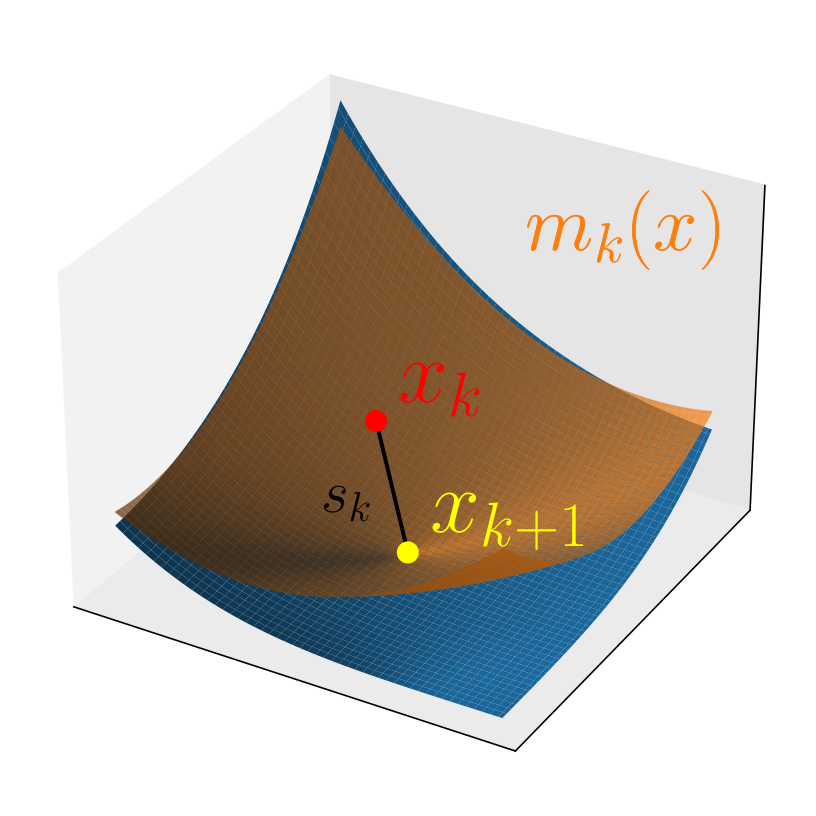
\includegraphics[width=\columnwidth]{../imgs/quasi_newton/quasi_newton_2.png}
    \end{minipage}%
    \begin{minipage}{0.33\columnwidth}
        \centering
        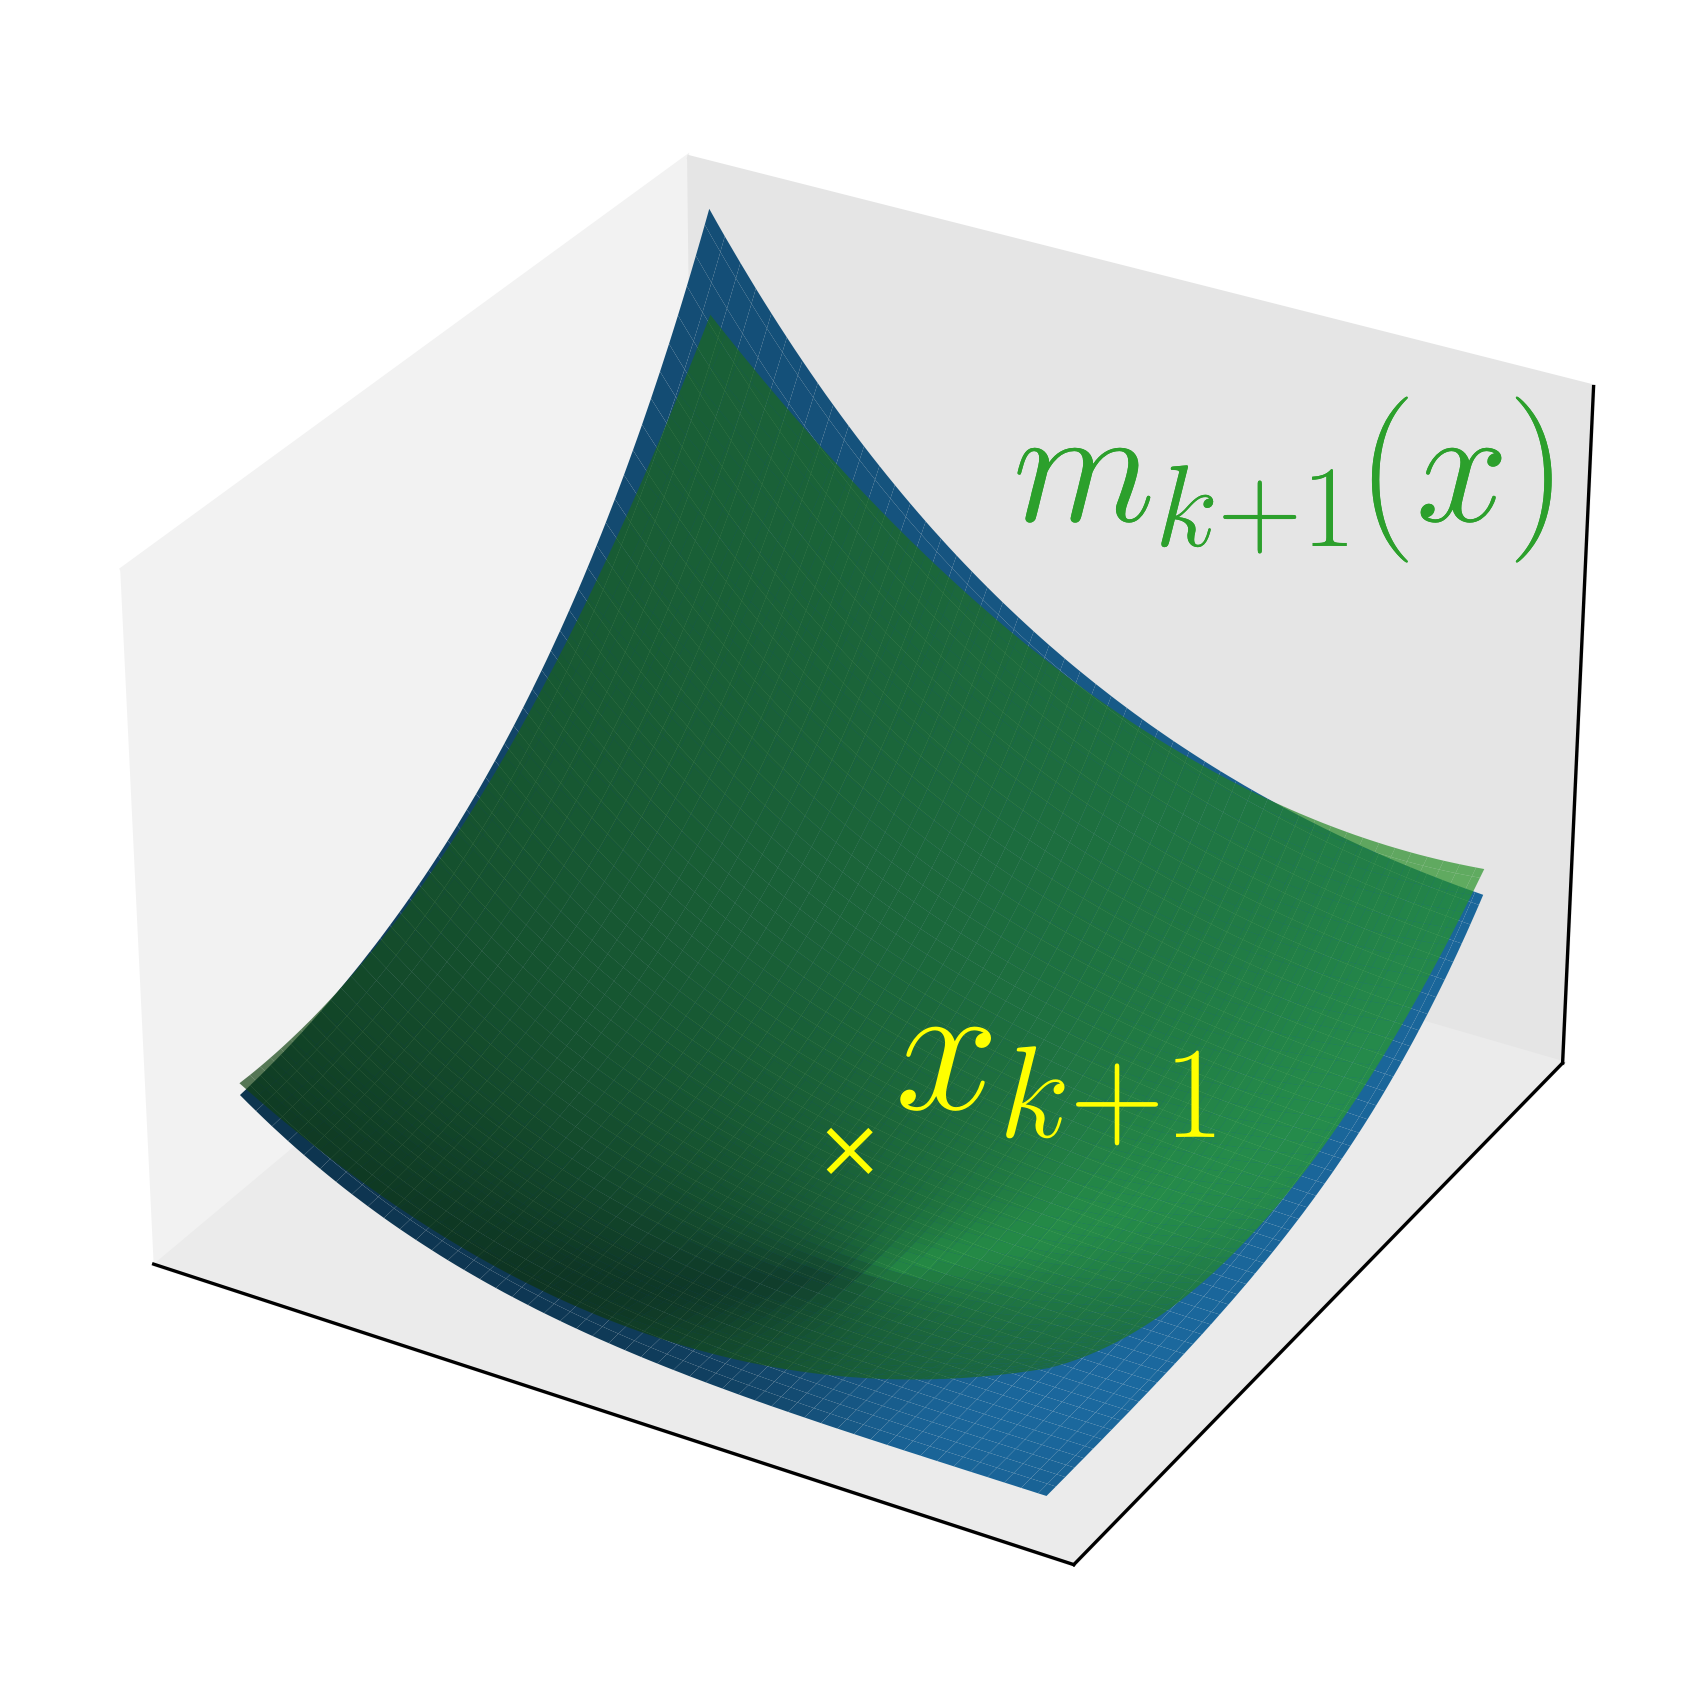
\includegraphics[width=\columnwidth]{../imgs/quasi_newton/quasi_newton_3.png}
    \end{minipage}
    \caption{
        準Newton法の概念図。
        (1) 目的関数 $f$(青い曲面) と現在の点 $x_k$(赤点) 。
        (2) 現在のヘッセ行列近似による二次モデル(オレンジの曲面) とその最小点 $x_{k+1}$(黄色の十字) 。
        (3) 新しい点 $x_{k+1}$ に基づいて更新された二次モデル(緑の曲面) 。
    }
    \label{fig:quasi_newton_overview}
\end{figure}

準Newton法の核心は、各反復において $B_k$(またはその逆行列 $H_k$) をどのように更新し、ヘッセ行列 $\nabla^2 f(x_k)$ に近づけるかにある。
\Cref{fig:quasi_newton_overview}にその概念図を示す。
まず、現在の点 $x_k$ のまわりで、$B_k$ を用いて目的関数 $f$ の二次近似モデルを構築する。
次に、この二次モデルを最小化して次の点 $x_{k+1}$ を求める。
点 $x_{k+1}$ を得た後、ステップ $s_k \coloneqq x_{k+1} - x_k$ および勾配の変化 $y_k \coloneqq \nabla f(x_{k+1}) - \nabla f(x_k)$ の情報を用いて、近似行列 $B_k$ を $B_{k+1}$ に更新する。
この手続きを収束するまで繰り返すのが準Newton法である。

以下では、近似ヘッセ行列 $B_k$が満たすべきとされるセカント条件を導入し、そのような条件を満たすような $B_k$ および $H_k$ に対するいくつかの代表的な更新則を紹介する。

\subsection{セカント条件(Secant Condition) }

本節でも、$f\colon \bbR^n \to \bbR$ を $C^2$ 級の関数とする。ヘッセ行列 $\nabla^2 f(x_k)$ の近似として対称行列 $B_k$ が与えられているとき、次の点 $x_{k+1}$ におけるヘッセ行列の近似 $B_{k+1}$ を求めたい。

このような行列の候補は無数に存在するが、ヘッセ行列が対称であることを考慮し、$B_{k+1}$ も対称であることを課すのは自然である。

ここで、$\nabla f(x_k)$ のテイラー展開を用いると、
\begin{align*}
    \nabla f(x_k) & = \nabla f(x_{k+1}) + \nabla^2 f(x_{k+1})(x_k - x_{k+1}) + \order{\norm{x_k - x_{k+1}}^2} \\
                  & \approx \nabla f(x_{k+1}) + \nabla^2 f(x_{k+1})(x_k - x_{k+1})                            \\
                  & \approx \nabla f(x_{k+1}) + B_{k+1}(x_k - x_{k+1})
\end{align*}
である。
ここで、$s_k \coloneqq x_{k+1} - x_k$、$y_k \coloneqq \nabla f(x_{k+1}) - \nabla f(x_k)$、および $\rho_k \coloneqq \frac{1}{y_k^\top s_k}$(ただし $y_k^\top s_k \neq 0$) と定義する。このとき、先の近似が等式として成り立つことを要求すれば、
\begin{equation*}
    B_{k+1}(x_{k+1} - x_k) = \nabla f(x_{k+1}) - \nabla f(x_k) \iff B_{k+1}s_k = y_k
\end{equation*}
という関係式が得られる。

この関係式をセカント条件(secant condition)、または準Newton方程式(quasi-Newton equation)と呼ぶ。

\subsection{代表的な準Newton更新則}

$B_k$, $s_k$, $y_k$, が与えられたとき、
セカント条件を満たすような $B_{k+1}$ を与える更新則はいくつも存在する。ここではいくつかの代表的なものを紹介する。

本小節に限り、簡潔のため、$B_k$, $B_{k+1}$, $s_k$, $y_k$, $\rho_k$ を、それぞれ $B$, $\bar{B}$, $s$, $y$, $\rho$ と略記する。

\subsubsection{SR1更新則}

SR1更新則 \cite{nocedal1999numerical}(\href{https://en.wikipedia.org/wiki/Symmetric_rank-one}{Wikipedia}) は次の式で与えられる:
\begin{align*}
    \bar{B}_{\mathrm{SR1}} & = B + \frac{(y - B s)(y - B s)^\top}{(y - B s)^\top s} \\
    \bar{H}_{\mathrm{SR1}} & = H + \frac{(s - H y)(s - H y)^\top}{(s - H y)^\top y}
\end{align*}

この更新則を導出する。ランク1の更新によって $\bar{B}$ を構築すると仮定する。すなわち、ある $z \in \bbR^n$ に対して $\bar{B}_{\mathrm{SR1}} = B + z z^\top$ とする。この更新がセカント条件$\bar{B}_{\mathrm{SR1}} s = y$を満たすためには、$z^\top s \neq 0$ として次が成り立たねばならない:
\begin{equation}\label{eq:sr1-derivation}
    B s + z z^\top s = y \iff z = \frac{y - B s}{z^\top s}
\end{equation}
\cref{eq:sr1-derivation}の表式において、$s$との内積を取ると、
\begin{equation}\label{eq:sr1-derivation2}
    z^\top s = \frac{(y - B s)^\top s}{z^\top s} \iff (z^\top s)^2 = (y - B s)^\top s
\end{equation}
が得られる。したがって、\cref{eq:sr1-derivation,eq:sr1-derivation2}を組み合わせると、
\begin{equation*}
    \bar{B}_{\mathrm{SR1}}
    = B + z z^\top
    = B + \frac{(y - B s)(y - B s)^\top}{(z^\top s)^2}
    = B + \frac{(y - B s)(y - B s)^\top}{(y - B s)^\top s}
\end{equation*}
と、SR1更新則が得られる。
なお、$(y - Bs)^\top s = 0$ の場合は、通常この更新をスキップする。

\subsubsection{PSB更新則}

PSB更新則 \cite{haeltermanAnalyticalStudyLeast2009} は次の式で与えられる:
\begin{equation*}
    \bar{B}_{\mathrm{PSB}} = B + \frac{(y - B s) s^\top + s (y - B s)^\top}{s^\top s} - \frac{s^\top (y - B s)}{(s^\top s)^2} s s^\top
\end{equation*}
\begin{equation*}
    \bar{H}_{\mathrm{PSB}} = H + \frac{(s - H y) y^\top + y (s - H y)^\top}{y^\top y} - \frac{y^\top (s - H y)}{(y^\top y)^2} y y^\top
\end{equation*}

SR1では、初めから対称性を維持するために $z z^\top$ を加える形でランク1更新を行った。しかし、対称性を一時的に破ることを許し、$z c^\top$ の形でランク1更新を行うことも考えられる。ある $c \in \bbR^n$ に対して、
\begin{equation*}
    z = \frac{y - B s}{c^\top s}
\end{equation*}
とすれば、
\begin{equation*}
    C_1 \coloneqq B + \frac{(y - B s)c^\top}{c^\top s}
\end{equation*}
と更新できる。$C_1$ は一般に対称ではないため、次に対称化を行う:
\begin{equation*}
    C_2 = \frac{C_1 + C_1^\top}{2}
\end{equation*}
しかし、$C_2$ が必ずしもセカント条件を満たすとは限らないため、この操作を繰り返す:
\begin{equation*}
    \begin{dcases}
        C_0 = B                                                  \\
        C_{2t+1} = C_{2t} + \frac{(y - C_{2t}s)c^\top}{c^\top s} \\
        C_{2t+2} = \frac{C_{2t+1} + C_{2t+1}^\top}{2}
    \end{dcases}
\end{equation*}
このように定義される列 $\{ C_t \}_{t=0}^{\infty}$ は収束し、その極限は以下で示すように対称なセカント条件を満たす行列となる。

\begin{proposition}
    列 $\{ C_{2t} \}_{t=0}^{\infty}$ は収束し、その極限は次式で与えられる:
    \begin{equation*}
        \lim_{t \to \infty} C_{2t}
        = B + \frac{(y - Bs)c^\top + c(y - Bs)^\top}{c^\top s} - \frac{(y - Bs)^\top s}{(c^\top s)^2} c c^\top
    \end{equation*}
\end{proposition}
\begin{proof}
    2ステップをまとめて考えると次が得られる:
    \begin{equation*}
        C_{2t+2} = \frac{C_{2t+1} + C_{2t+1}^\top}{2}
        = C_{2t}
        + \frac{1}{2}
        \frac{(y - C_{2t}s)c^\top + c(y - C_{2t}s)^\top}{c^\top s}
    \end{equation*}
    よって
    \begin{align*}
        \lim_{t \to \infty} C_{2t}
         & = B + \sum_{t=0}^{\infty} \frac{1}{2} \frac{(y - C_{2t}s)c^\top + c(y - C_{2t}s)^\top}{c^\top s}                                 \\
         & = B + \frac{1}{2 c^\top s} \qty(\qty(\sum_{t=0}^{\infty} (y - C_{2t}s)) c^\top + \qty(\sum_{t=0}^{\infty} (y - C_{2t}s))^\top c)
    \end{align*}
    さらに次が成り立つ:
    \begin{align*}
        y - C_{2(t+1)}s
         & = y - \qty(C_{2t}
        + \frac{1}{2}
        \frac{(y - C_{2t}s)c^\top + c(y - C_{2t}s)^\top}{c^\top s})s   \\
         & = \frac{1}{2}
        \qty(I - \frac{c s^\top}{c^\top s})
        (y - C_{2t}s)                                                  \\
         & = \frac{1}{2} \qty(I - \frac{c s^\top}{c^\top s}) (y - B s)
    \end{align*}
    よって
    \begin{align*}
                                                                                        & \sum_{t=0}^{\infty} (y - C_{2t}s)                                                                              \\
        = {}                                                                            & \sum_{t=0}^{\infty} \frac{1}{2^t} \qty(I - \frac{c s^\top}{c^\top s})^t (y - B s)                              \\
        = {}                                                                            &
        y - B s+
        \sum_{t=1}^{\infty} \frac{1}{2^t} \qty(I - \frac{c s^\top}{c^\top s}) (y - B s) &                                                                                   & (\text{idempotent matrix}) \\
        = {}                                                                            & y - B s + (I-\frac{c s^\top}{c^\top s})(y - B s)                                                               \\
        ={}                                                                             & \qty(2I - \frac{c s^\top}{c^\top s})(y - Bs)
    \end{align*}
    よって次が得られる:
    \begin{align*}
        \lim_{t \to \infty} C_{2t}
         & = B + \frac{1}{2 c^\top s} \qty(\qty(\sum_{t=0}^{\infty} (y - C_{2t}s)) c^\top + \qty(\sum_{t=0}^{\infty} (y - C_{2t}s))^\top c)           \\
         & = B + \frac{1}{2 c^\top s} \qty(\qty(2I - \frac{c s^\top}{c^\top s})(y - Bs) c^\top + \qty(2I - \frac{c s^\top}{c^\top s})(y - Bs)^\top c) \\
         & = B
        + \frac{(y - Bs)c^\top + c(y - Bs)^\top}{c^\top s}
        - \frac{(y - Bs)^\top s}{(c^\top s)^2} c c^\top
    \end{align*}
\end{proof}

ここで $c=s$ とすると:
\begin{equation}\label{eq:PSB_update}
    \bar{B}_{\mathrm{PSB}} = B + \frac{(y - Bs)s^\top + s(y - Bs)^\top}{s^\top s} - \frac{(y - Bs)^\top s}{(s^\top s)^2} ss^\top
\end{equation}

この更新則は Powell Symmetric Broyden (PSB) 更新則と呼ばれる。

Powell(1970d) は、Broyden法の二重ランク版を導出する手法を提案した。
Dennis(1972) は、Powellの手法により、ほとんどの既知の準ニュートン更新則を導出できることを示した。

\subsubsection{DFP Update}

The DFP update \cite{nocedal1999numerical} (\href{https://en.wikipedia.org/wiki/Davidon%E2%80%93Fletcher%E2%80%93Powell_formula}{Wikipedia}) is given by the following update formulas:
\begin{equation*}
    \bar{B}_{\mathrm{DFP}} = (I - \rho y s^\top) B (I - \rho s y^\top) + \rho y y^\top
\end{equation*}
\begin{equation*}
    \bar{H}_{\mathrm{DFP}} = H - \frac{H y y^\top H}{y^\top H y} + \frac{s s^\top}{y^\top s}
\end{equation*}

\cite[Section 4.4]{haeltermanAnalyticalStudyLeast2009}

% Column-Updating method
% Pearson's method 172
% McCormick's method 172
% The Eirola--Nevanlinna method

% https://en.wikipedia.org/wiki/Compact_quasi-Newton_representation

% QUASI-NEWTON METHODS, MOTIVATION AND THEORY
% Section 7

In the PSB update rule discussed earlier, we substituted $c=s$, but we can consider taking a different $c$. Specifically, we consider choosing $c$ such that $B_{k+1}$ becomes positive definite.

In conclusion, substituting $c=y$ makes this positive definite, and we obtain:
\begin{equation}\label{eq:DFP_rank}
    \bar{B}_{\mathrm{DFP}} = B + \frac{(y - Bs)y^\top + y(y - Bs)^\top}{y^\top s} - \frac{(y - Bs)^\top s}{(y^\top s)^2} yy^\top
\end{equation}

This is called the Davidon--Fletcher--Powell (DFP) update.

Lemma 7.4.

対称行列 $A \in \bbR^n$が
$$
    \lambda_1 \leq \lambda_2 \leq \dots \leq \lambda_n
$$
と固有値を持つとします。
ある $u \in \bbR^n$ に対して $A^* = A + \sigma uu^\top$ とし、その固有値を$\lambda_i^*$とします。
この時、$\sigma > 0$ ならば
$$
    \lambda_1 \leq \lambda_1^{*} \leq \lambda_2 \dots \leq \lambda_n \leq \lambda_n^{*}
$$
であり、$\sigma < 0$ ならば
$$
    \lambda_1^{*} \leq \lambda_1 \leq \lambda_2^* \dots \leq \lambda_n^{*} \leq \lambda_n
$$
が成り立つ。

Cauchy's Interlacing Theoremの亜種として知られているようです。

https://simple-complexities.github.io/eigenvalue/interlacing/2020/02/10/interlacing.html

\begin{theorem}[Cauchyの交錯定理 (Cauchy's interlacing theorem)]
    $B$ を実対称行列とし、次を定義します。
    \begin{equation*}
        A = B + \bm{x}\bm{x}^{T}.
    \end{equation*}
    $A$ の固有値を $\lambda_1 \ge \cdots \ge \lambda_n$、$B$ の固有値を $\mu_1 \ge \cdots \ge \mu_n$ とすると、これらは次のように交錯しています。
    \begin{equation*}
        \lambda_1 \ge \mu_1 \ge \lambda_2 \ge \mu_2 \ge \cdots \ge \lambda_n \ge \mu_n.
    \end{equation*}
\end{theorem}
\begin{proof}
    任意の $\bm{y} \in \bbR^n$ に対して、
    \begin{equation*}
        \bm{y}^\top A \bm{y} = \bm{y}^\top B \bm{y} + \bm{y}^\top \bm{x} \bm{x}^\top \bm{y}
        \geq \bm{y}^\top B \bm{y}.
    \end{equation*}

    固有値のレイリー商表現(Rayleigh quotient characterization)は次の通りです。
    \begin{align*}
        \lambda_i & = \max_{U \le \bbR^n,\ \dim U = i} \ \min_{\bm{y} \in U, |\bm{y}| = 1} (\bm{y}^\top A \bm{y}), \\
        \mu_i     & = \max_{U \le \bbR^n,\ \dim U = i} \ \min_{\bm{y} \in U, |\bm{y}| = 1} (\bm{y}^\top B \bm{y}).
    \end{align*}
    $\bm{y}^\top A \bm{y} \ge \bm{y}^\top B \bm{y}$ が任意の $\bm{y}$ で成り立つので、関数 $f \ge g$ が共通の定義域上で成り立つとき、
    $\min f \ge \min g$ および $\max f \ge \max g$ が成立します。これを二度適用すれば $\lambda_i \ge \mu_i$ が従います。

    次の $(n-1)$ 次元部分空間を定義します。
    \begin{equation*}
        V = \{\bm{y} \in \bbR^n \mid \bm{x}^\top \bm{y} = 0\}.
    \end{equation*}

    $\bbR^n$ の $i$ 次元部分空間 $U$ を考え、次を定義します。
    \begin{equation*}
        U' = U \cap V.
    \end{equation*}

    このとき $\dim(U')$ は $i-1$ または $i$ です。
    これは次の一般的な関係式から従います。
    \begin{equation*}
        n \ge \dim(U + V) = \dim(U) + \dim(V) - \dim(U \cap V),
    \end{equation*}
    したがって $\dim(U') \le \dim(U)$ です。

    任意の $\bm{y} \in U'$ に対して、
    \begin{align*}
        \bm{y}^\top A \bm{y} & = \bm{y}^\top B \bm{y} + \bm{y}^\top \bm{x}\bm{x}^\top \bm{y} \\
                             & = \bm{y}^\top B \bm{y} + (\bm{x}^\top \bm{y})^2               \\
                             & = \bm{y}^\top B \bm{y},
    \end{align*}
    が成り立ちます。

    したがって、部分集合上での最小値は上位集合上での最小値より小さくはなりませんから、
    \begin{equation*}
        \min_{\bm{y} \in U'} \bm{y}^\top B \bm{y} = \min_{\bm{y} \in U'} \bm{y}^\top A \bm{y} \ge \min_{\bm{y} \in U} \bm{y}^\top A \bm{y}.
    \end{equation*}

    さらに、
    \begin{equation*}
        \mu_i = \max_{S \le \bbR^n,\ \dim S \ge i} \min_{\bm{y} \in S, |\bm{y}| = 1} \bm{y}^\top B \bm{y} \ge \min_{\bm{y} \in U'} \bm{y}^\top B \bm{y} \ge \min_{\bm{y} \in U} \bm{y}^\top A \bm{y}
    \end{equation*}
    が全ての $U$ に対して成り立ちます($\dim S = i$ を $\dim S \ge i$ に置き換えても結果は変わりません)。

    よって、
    \begin{equation*}
        \mu_i \ge \max_{U \le \bbR^n,\ \dim U = i+1} \min_{\bm{y} \in U} \bm{y}^\top A \bm{y} = \lambda_{i+1}.
    \end{equation*}

    これで証明は完了です。
\end{proof}

定理7.5.
正定値対称行列 $B \in \bbR^n$、$c, s, y_k \in \bbR^n$ で $(c, s) \neq 0$ とします。このとき、(7.9) により定義される $B$ が正定値であるのは、$\det B > 0$ である場合に限ります。

証明. $B$ が正定値であれば、明らかに $\det B > 0$ です。逆を示すには、まず $B$ を以下のように書けることに注目します:
$$
    B = B_{k+1} + vw^\top + wv^\top,
$$
ここで $v = c$ であり、
$$
    w = \frac{y_k - B_{k+1}s}{2(c, s)}
$$
です。したがって、
$$
    B = B_{k+1} + 2\left[(v + w)(v + w)^\top - (v - w)(v - w)^\top\right]
$$
と表せるので、$B$ は $B_{k+1}$ に2つの対称なランク1行列の和を加えた形で表現されます。

$B_{k+1}$ が正定値であれば、補題7.4より、$B$ は高々1つの非正の固有値しか持ち得ません。よって、$\det B > 0$ であれば、全ての固有値は正となり、$B$ は正定値です。

定理7.5から、(7.9) により定義される更新式が (7.1) および (7.14) を満たすためには、$B$ が対称かつ正定値であるときに $\det B > 0$ が成り立つ必要があります。この要件を満たす $c$ の選び方を知るためには、$\det B$ の表現が必要です。

**補題7.6.** $u_i \in \bbR^n$($i = 1, 2, 3, 4$)とします。このとき
$$
    \det(I + u_1 u_2^\top + u_3 u_4^\top) = (1 + (u_1, u_2))(1 + (u_3, u_4)) - (u_1, u_4)(u_2, u_3)
$$
が成り立ちます。

**証明.** この結果の証明は Pearson (1969) にありますが、以下は代替の議論です。

一時的に $(u_1, u_2) \neq -1$ と仮定します。このとき $I + u_1 u_2^\top$ は可逆であり、
$$
    I + u_1 u_2^\top + u_3 u_4^\top = (I + u_1 u_2^\top)\qty(I + (I + u_1 u_2^\top)^{-1} u_3 u_4^\top)
$$
と書けます。この結果は補題4.2および4.4を用いることで導かれます。$(u_1, u_2) \neq -1$ の場合に成り立つので、連続性の議論により一般にも成り立つことが示されます。

(7.9) に補題7.6を適用します。いくつかの代数的操作により、次が得られます:
\begin{equation*}
    \det B = \det B_{k+1} \left[\frac{(c, H y)^2 - (c, H c)(y, H y) + (c, H c)(y, s)}{(c, s)^2}\right]
\end{equation*}

ここで $H = B_{k+1}^{-1}$ です。$B_{k+1}$ が正定値であると仮定し、$v = H^{1/2} y$、$w = H^{1/2} c$ とおくと、
\begin{equation}
    \det B = \det B_{k+1} \left[\frac{(v, w)^2 - \|v\|^2 \|w\|^2 + \|w\|^2 (y, s)}{(c, s)^2}\right] \tag{7.16}
\end{equation}
となります。定理7.5により、$B$ が正定値であるのは次のときに限ります:
\begin{equation}
    \|w\|^2 (y, s) > \|v\|^2 \|w\|^2 - (v, w)^2. \tag{7.17}
\end{equation}

この不等式 (7.17) を自然に満たす最も簡単な方法は、$w$ を $v$ のスカラー倍にすることです。この場合、(7.17) は単に $(y, s)$ が正であることを要求するだけになります。このとき、$c$ は $y$ のスカラー倍となり、(7.9) は Davidon (1959) によって導入された更新式に帰着します。

Derivation of the Inverse Update

$$
    H' = H + \frac{(s_k - Hy)(s_k - Hy)^\top}{(s_k - Hy, y)}
$$

特徴づけ

\subsubsection{BFGS 更新則}

Broyden--Fletcher--Goldfarb--Shanno

\cite{nocedal1999numerical}

% https://en.wikipedia.org/wiki/Broyden%E2%80%93Fletcher%E2%80%93Goldfarb%E2%80%93Shanno_algorithm

\begin{equation*}
    \bar{B}_{\mathrm{BFGS}} = B - \frac{B s s^\top B}{s^\top B s} + \frac{y y^\top}{y^\top s}
\end{equation*}
\begin{equation*}
    \bar{H}_{\mathrm{BFGS}} = \qty(I - \rho s y^\top) H \qty(I - \rho y s^\top) + \rho s s^\top
\end{equation*}
\begin{equation*}
    \rho = \frac{1}{y^\top s}
\end{equation*}

DFPとBFGSは双対的な関係にある。

詳細は後述する。

\subsubsection{Broyden Family}
\begin{equation*}
    B_{k+1} = B_k - \frac{B_k s_k s_k^\top B_k}{s_k^\top B_k s_k} + \frac{y_k y_k^\top}{y_k^\top s_k} + \varphi_k (s_k^\top B_k s_k) v_k v_k^\top
\end{equation*}
\begin{equation*}
    v_k = \frac{y_k}{y_k^\top s_k} - \frac{B_k s_k}{s_k^\top B_k s_k}
\end{equation*}

\subsection{BFGS Method}

\subsubsection{Basic Notation}

Let $f\colon \bbR^n \to \bbR$ be a twice continuously differentiable function.
Let $x_k$ denote the $k$-th iterate, and let $B_k$ denote the approximation of the Hessian $\nabla^2 f(x_k)$ at iteration $k$.
Define the step and gradient difference as
\begin{align}
    s_k & = x_{k+1} - x_k, \label{eq:step}                              \\
    y_k & = \nabla f(x_{k+1}) - \nabla f(x_k), \label{eq:gradient_diff}
\end{align}
where we assume that $y_k^\top s_k \neq 0$.
Here, the $s$ in $s_k$ stands for \emph{step}.
We also define $\rho_k = (y_k^\top s_k)^{-1}$.

\subsubsection{BFGS update}\label{sec:BFGS_update}

The following two algebraically equivalent forms of the BFGS update are widely used:
\begin{equation}\label{eq:Bk_rank}
    B_{k+1}   = B_k - \frac{B_k s_k s_k^\top B_k}{s_k^\top B_k s_k} + \frac{y_k y_k^\top}{y_k^\top s_k}.
\end{equation}
The \emph{rank-two update form}.

\subsubsection{Formula for \texorpdfstring{$H_k$}{Hk}}

The inverse of the BFGS update $H_k \defeq B_k^{-1}$ also has two equivalent forms:
\begin{equation}
    H_{k+1} = (I - \rho_k s_k y_k^\top) H_k (I - \rho_k y_k s_k^\top) + \rho_k s_k s_k^\top. \label{eq:Hk_compact}
\end{equation}

\begin{proposition}
    \Cref{eq:Hk_compact} gives the exact inverse of the BFGS update, i.e., $H_{k+1} = B_{k+1}^{-1}$.
\end{proposition}

\begin{proof}
    Define
    \begin{equation*}
        U =
        \begin{bmatrix}
            B_k s_k & y_k
        \end{bmatrix}
        \in \bbR^{n\times 2},
        \qquad
        M =
        \begin{pmatrix}
            -1/s_k^\top B_k s_k & 0              \\
            0                   & 1/y_k^\top s_k
        \end{pmatrix}.
    \end{equation*}
    Then
    \begin{equation*}
        U M U^\top
        = -\frac{1}{s_k^\top B_k s_k}(B_k s_k)(B_k s_k)^\top
        + \frac{1}{y_k^\top s_k} y_k y_k^\top \\
        = -\frac{B_k s_k s_k^\top B_k}{s_k^\top B_k s_k}
        + \frac{y_k y_k^\top}{y_k^\top s_k},
    \end{equation*}
    and hence the BFGS update can be written compactly as
    \begin{equation*}
        B_{k+1} = B_k + U M U^\top.
    \end{equation*}

    Now, by the Sherman--Morrison--Woodbury formula, for any invertible matrix $A$,
    \begin{equation*}
        (A + U C V)^{-1}
        = A^{-1} - A^{-1} U \bigl(C^{-1} + V A^{-1} U\bigr)^{-1} V A^{-1}.
    \end{equation*}
    Applying this identity with $A = B_k$, $C = M$, and $V = U^\top$, we obtain
    \begin{equation*}
        B_{k+1}^{-1}
        = (B_k + U M U^\top)^{-1}
        = H_k - H_k U \bigl(M^{-1} + U^\top H_k U\bigr)^{-1} U^\top H_k.
    \end{equation*}

    Since $B_k H_k = I$, it follows that
    \begin{equation*}
        M^{-1} + U^\top H_k U
        =
        \begin{pmatrix}
            -s_k^\top B_k s_k & 0            \\
            0                 & y_k^\top s_k
        \end{pmatrix}
        +
        \begin{pmatrix}
            s_k^\top B_k s_k & s_k^\top y_k     \\
            s_k^\top y_k     & y_k^\top H_k y_k
        \end{pmatrix}
        =
        \begin{pmatrix}
            0            & s_k^\top y_k                    \\
            s_k^\top y_k & y_k^\top H_k y_k + s_k^\top y_k
        \end{pmatrix}.
    \end{equation*}

    The inverse of this $2 \times 2$ matrix is
    \begin{equation*}
        (M^{-1} + U^\top H_k U)^{-1}
        =
        \frac{1}{(s_k^\top y_k)^2}
        \begin{pmatrix}
            -\bigl(y_k^\top H_k y_k + s_k^\top y_k\bigr) & s_k^\top y_k \\
            s_k^\top y_k                                 & 0
        \end{pmatrix}.
    \end{equation*}
    Recalling $\rho_k = 1 / (y_k^\top s_k)$, we can rewrite this as
    \begin{equation*}
        (M^{-1} + U^\top H_k U)^{-1}
        =
        \begin{pmatrix}
            -\rho_k^2 (y_k^\top H_k y_k) - \rho_k & \rho_k \\
            \rho_k                                & 0
        \end{pmatrix}.
    \end{equation*}

    Substituting the above result, we obtain
    \begin{align*}
        B_{k+1}^{-1}
         & = H_k
        - \begin{bmatrix} s_k & H_k y_k \end{bmatrix}
        \begin{pmatrix}
            -\rho_k^2 (y_k^\top H_k y_k) - \rho_k & \rho_k \\
            \rho_k                                & 0
        \end{pmatrix}
        \begin{bmatrix} s_k^\top \\ y_k^\top H_k \end{bmatrix} \\
         & = H_k
        + \rho_k^2 (y_k^\top H_k y_k) s_k s_k^\top
        + \rho_k s_k s_k^\top
        - \rho_k s_k (y_k^\top H_k)
        - \rho_k (H_k y_k) s_k^\top.
    \end{align*}

    Finally, rearranging terms yields
    \begin{equation*}
        H_{k+1}
        = (I - \rho_k s_k y_k^\top) H_k (I - \rho_k y_k s_k^\top)
        + \rho_k s_k s_k^\top,
    \end{equation*}
    which is precisely the desired compact form. Hence,
    \begin{equation*}
        H_{k+1} = B_{k+1}^{-1}.
    \end{equation*}
\end{proof}



We can verify that the compact form \cref{eq:Hk_compact} gives the exact inverse of the BFGS update, i.e., $H_{k+1} = B_{k+1}^{-1}$, as follows.

First, note the following two key relations obtained directly from \cref{eq:Bk_rank} and \cref{eq:Hk_compact}:
\begin{align}
    B_{k+1} s_k & = B_k s_k - \frac{B_k s_k s_k^\top B_k s_k}{s_k^\top B_k s_k} + \frac{y_k y_k^\top s_k}{y_k^\top s_k} = y_k, \label{eq:rel1} \\
    H_{k+1} y_k & = H_k y_k - \frac{H_k y_k y_k^\top H_k y_k}{y_k^\top H_k y_k} + \frac{s_k s_k^\top y_k}{s_k^\top y_k} = s_k. \label{eq:rel2}
\end{align}

Let $A \defeq H_{k+1} B_{k+1} - I$.
Both $B_{k+1}$ and $H_{k+1}$ are rank-two updates of $B_k$ and $H_k$, respectively, hence $\operatorname{rank}(A) \le 2$.
From \cref{eq:rel1,eq:rel2} we have
\begin{equation*}
    A s_k = (H_{k+1} B_{k+1} - I) s_k = H_{k+1} y_k - s_k = 0, \qquad
    y_k^\top A = 0^\top.
\end{equation*}
Thus $A$ annihilates both $s_k$ and $y_k$.
Since $\operatorname{rank}(A) \le 2$ and $\{s_k, y_k\}$ are linearly independent (because $y_k^\top s_k \neq 0$), we must have $A = 0$, i.e.,
\[
    H_{k+1} B_{k+1} = I.
\]
Hence, \cref{eq:Hk_compact} indeed gives the inverse of the BFGS update. The validity of the rank-two update form \cref{eq:Bk_rank} can be shown by a similar argument.

We can also verify by using the Sherman--Morrison--Woodbury (SMW) identity.
Recall that for any invertible matrix $A$ and vectors $u,v$, the inverse of a rank-one update is
\begin{equation}
    (A + u v^\top)^{-1} = A^{-1} - \frac{A^{-1} u v^\top A^{-1}}{1 + v^\top A^{-1} u}.
\end{equation}

\subsubsection{KL}

Let the function $\psi\colon \mathrm{PD}(n) \to \bbR$ be defined as
\begin{equation*}
    \psi(A) = \tr(A) - \log \det(A)
\end{equation*}

Then, the BFGS update can be written as
\begin{mini*}
    {B \in \mathrm{PD}(n)}
    {\psi(B_k^{-1/2} B B_k^{-1/2})}
    {\label{eq:bfgs-kl}}{}
    \addConstraint{Bs_k}{= y_k}
\end{mini*}

Kullback--Leibler(KL) divergence:
\begin{equation*}
    % \psi(A) = \tr(A) - \log \det(A)
    \mathrm{KL}(P,Q) \coloneqq \tr(P Q^{-1}) - \log \det(P Q^{-1}) - n
\end{equation*}
Under the secant equation constraint,
\begin{gather*}
    B_{k+1} = \arg\min_{B \in \mathrm{PD}(n)} \mathrm{KL}(B_k, B), \quad \text{(DFP)}\\
    B_{k+1} = \arg\min_{B \in \mathrm{PD}(n)} \mathrm{KL}(B, B_k). \quad \text{(BFGS)}
\end{gather*}
\begin{figure}[htbp]
    \centering
    \includegraphics[width=0.5\columnwidth]{../imgs/paperScreenShots/kanamori.png}
\end{figure}

Kullback--Leibler (KL) divergence between positive definite matrices \(P,Q\in\mathrm{PD}(n)\) is defined by
\[
    \mathrm{KL}(P,Q) \coloneqq \tr(P Q^{-1}) - \log\det(P Q^{-1}) - n.
\]

Under the secant equation constraint, the DFP and BFGS updates admit variational characterizations:
\[
    B_{k+1} = \arg\min_{B \in \mathrm{PD}(n)} \mathrm{KL}(B_k, B) \qquad\text{(DFP)},
\]
\[
    B_{k+1} = \arg\min_{B \in \mathrm{PD}(n)} \mathrm{KL}(B, B_k) \qquad\text{(BFGS)}.
\]

See Kanamori for an exposition of these formulations \citep{kanamoriBregmanExtensionQuasiNewton2010,kanamoriBregmanExtensionQuasiNewton2010a} (see also \href{http://matsuzoe.web.nitech.ac.jp/infogeo/OCAMI2010/kanamori.pdf}{Japanese slide}). Empirically, BFGS tends to be more numerically stable than DFP.

\citep{kanamoriBregmanExtensionQuasiNewton2010,kanamoriBregmanExtensionQuasiNewton2010a}

(\href{http://matsuzoe.web.nitech.ac.jp/infogeo/OCAMI2010/kanamori.pdf}{Japanese Slide})

BFGS tends to be more numerically stable than DFP.

\subsubsection{Determinant formula for BFGS update}

\[
    B_{+}=B-\frac{B s s^\top B}{s^\top B s}+\frac{y y^\top}{y^\top s}.
\]
Set
\[
    A \defeq B^{-1}\Big(-\frac{B s s^\top B}{s^\top B s}+\frac{y y^\top}{y^\top s}\Big)
    =-\frac{s s^\top B}{s^\top B s}+\frac{B^{-1}y\,y^\top}{y^\top s},
\]
so that
\[
    B_{+}=B(I+A).
\]
Hence
\begin{equation}
    \det(B_{+})=\det(B)\det(I+A).
\end{equation}
Note that $A$ is a rank--$2$ matrix and can be written in the form
\[
    A=u_1 v_1^\top+u_2 v_2^\top,
\]
with the choices
\[
    u_1=-s,\qquad v_1=\frac{B s}{s^\top B s},\qquad
    u_2=\frac{B^{-1}y}{y^\top s},\qquad v_2=y.
\]
Define the $n\times2$ matrices $U=[u_1\;u_2]$ and $V=[v_1\;v_2]$. Then $A=U V^\top$ and the matrix determinant lemma (in the form $\det(I+UV^\top)=\det(I_2+V^\top U)$) gives
\begin{equation}
    \det(I+A)=\det\big(I_2+V^\top U\big).
\end{equation}
Compute the $2\times2$ matrix $V^\top U$ entrywise:
\[
    V^\top U=
    \begin{pmatrix}
        v_1^\top u_1 & v_1^\top u_2 \\[4pt]
        v_2^\top u_1 & v_2^\top u_2
    \end{pmatrix}
    =
    \begin{pmatrix}
        -1         & \dfrac{s^\top y}{(s^\top B s)(y^\top s)} \\[8pt]
        - y^\top s & \dfrac{y^\top B^{-1}y}{y^\top s}
    \end{pmatrix}.
\]
Therefore
\[
    I_2+V^\top U=
    \begin{pmatrix}
        0          & \dfrac{s^\top y}{(s^\top B s)(y^\top s)} \\[8pt]
        - y^\top s & 1+\dfrac{y^\top B^{-1}y}{y^\top s}
    \end{pmatrix}.
\]
Its determinant is
\[
    \det(I_2+V^\top U)
    =0\cdot\Big(1+\frac{y^\top B^{-1}y}{y^\top s}\Big)
    -\frac{s^\top y}{(s^\top B s)(y^\top s)}\cdot(-y^\top s)
    =\frac{y^\top s}{s^\top B s}.
\]
Combining with $\det(B_{+})=\det(B)\det(I+A)$ yields the claimed identity
\[
    \boxed{\;\det(B_{+})=\det(B)\,\frac{y^\top s}{s^\top B s}\;},
\]
as required.

\subsection{BFGS vs DFP}

\href{https://link.springer.com/article/10.1007/BF01582161}{how bad}

\begin{figure}[htbp]
    \centering
    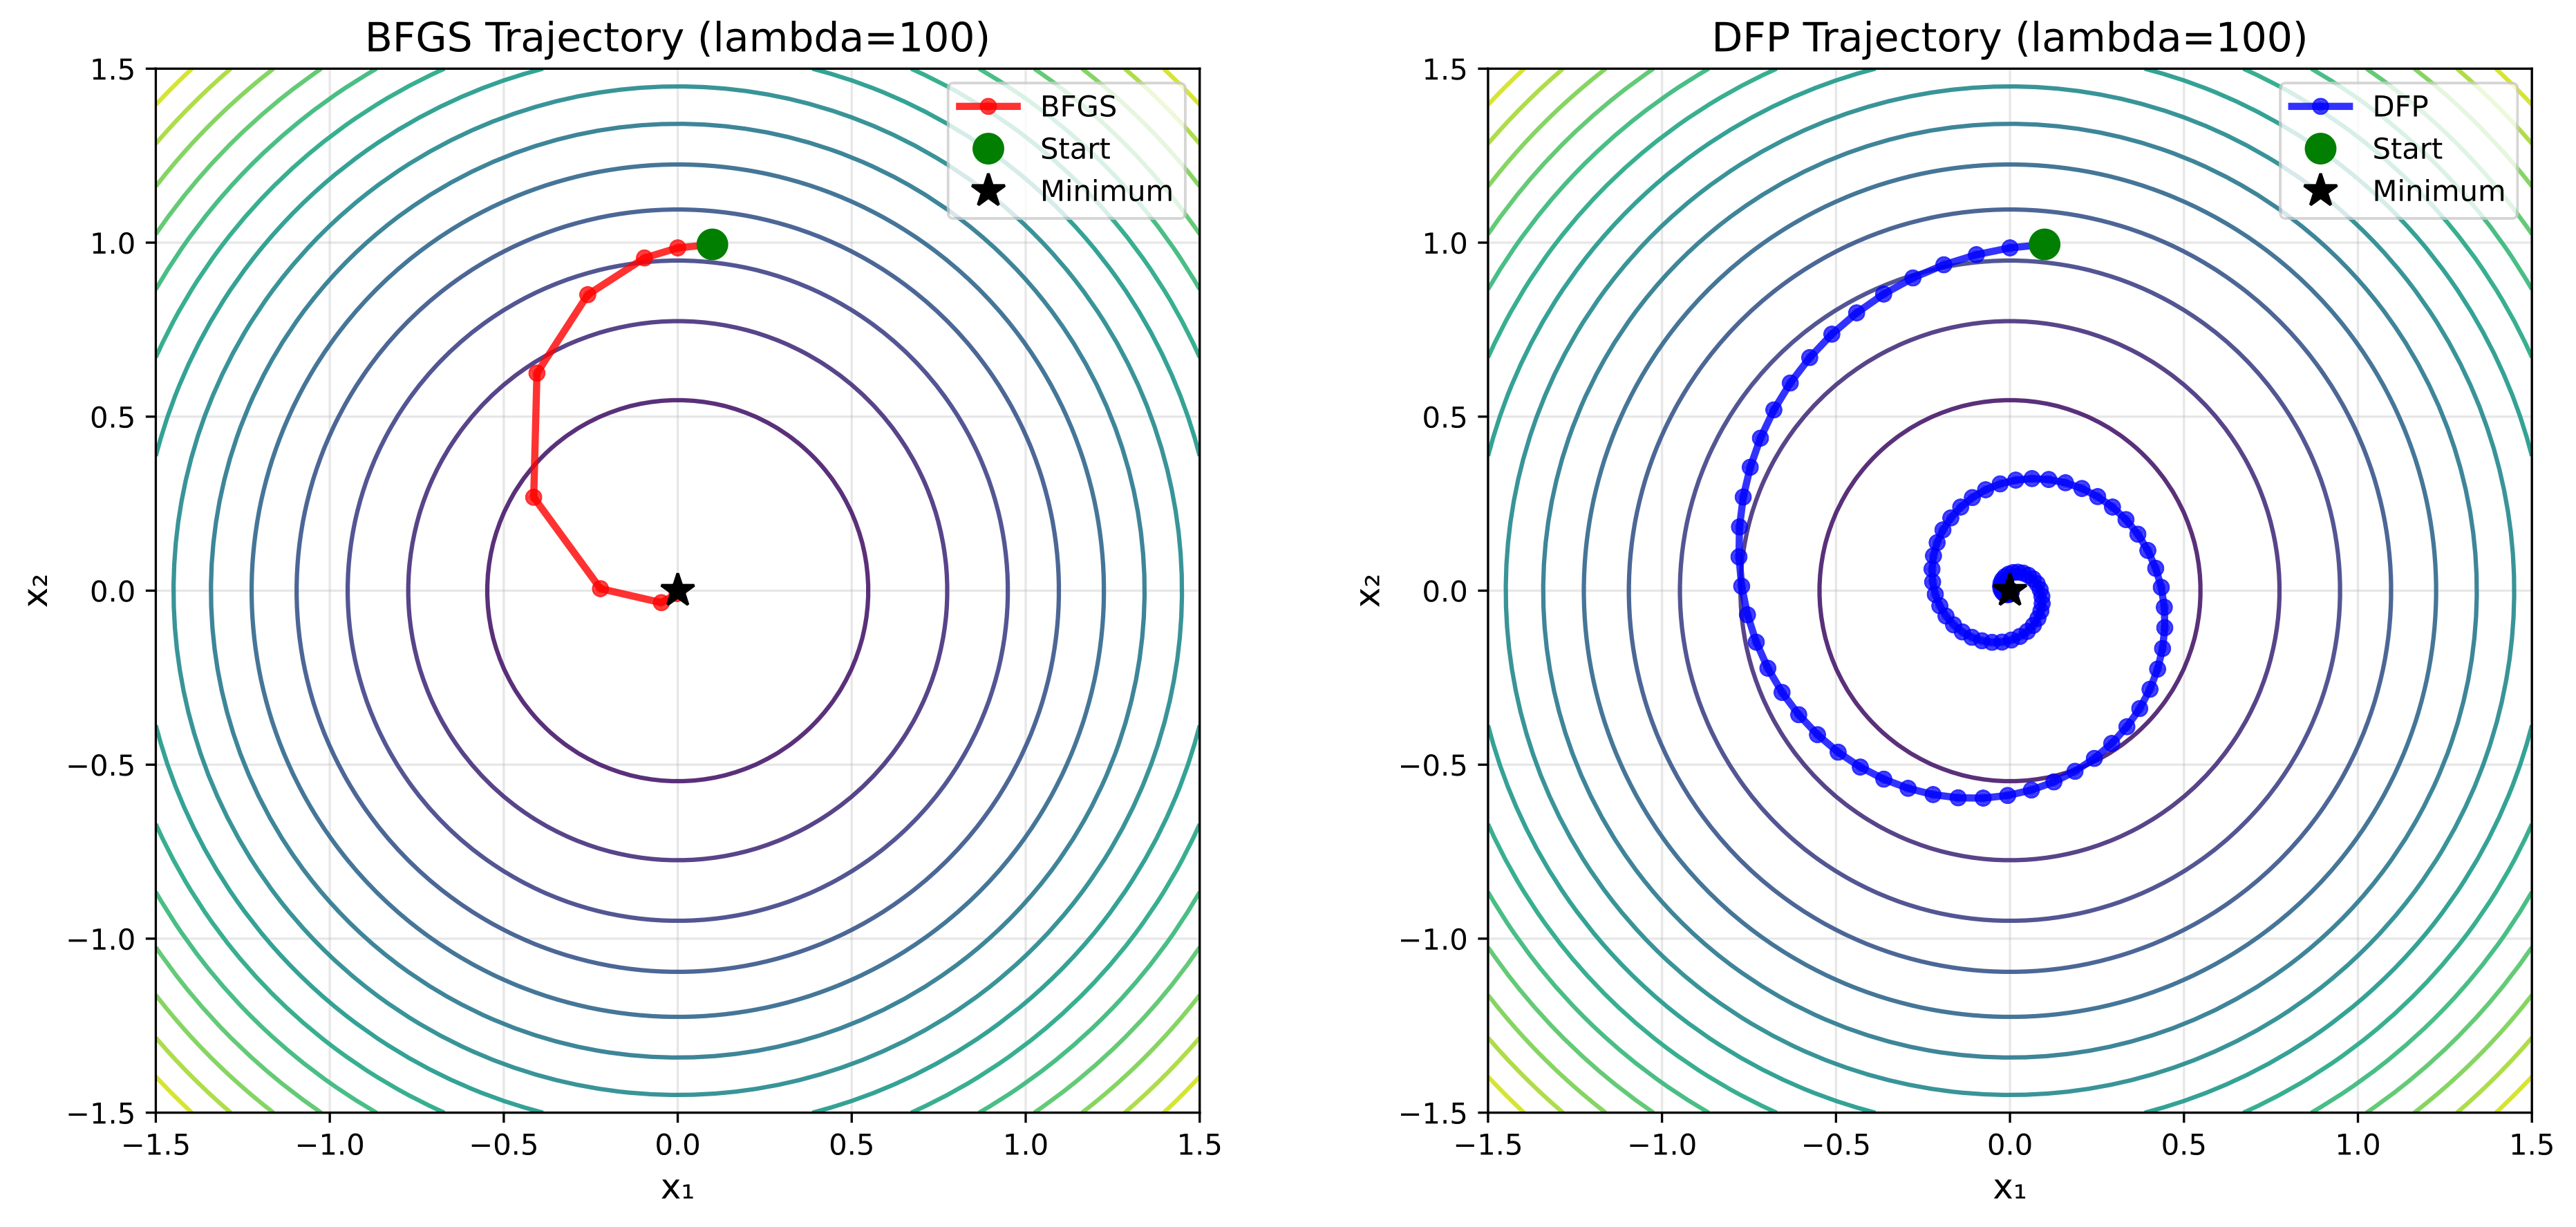
\includegraphics[width=\columnwidth]{../imgs/quasi_newton/bfgs_vs_dfp_100.png}
    \caption{BFGS と DFP の比較：$\lambda_1 = 100$}
    \label{fig:bfgs_vs_dfp_100}
\end{figure}

\begin{figure}[htbp]
    \centering
    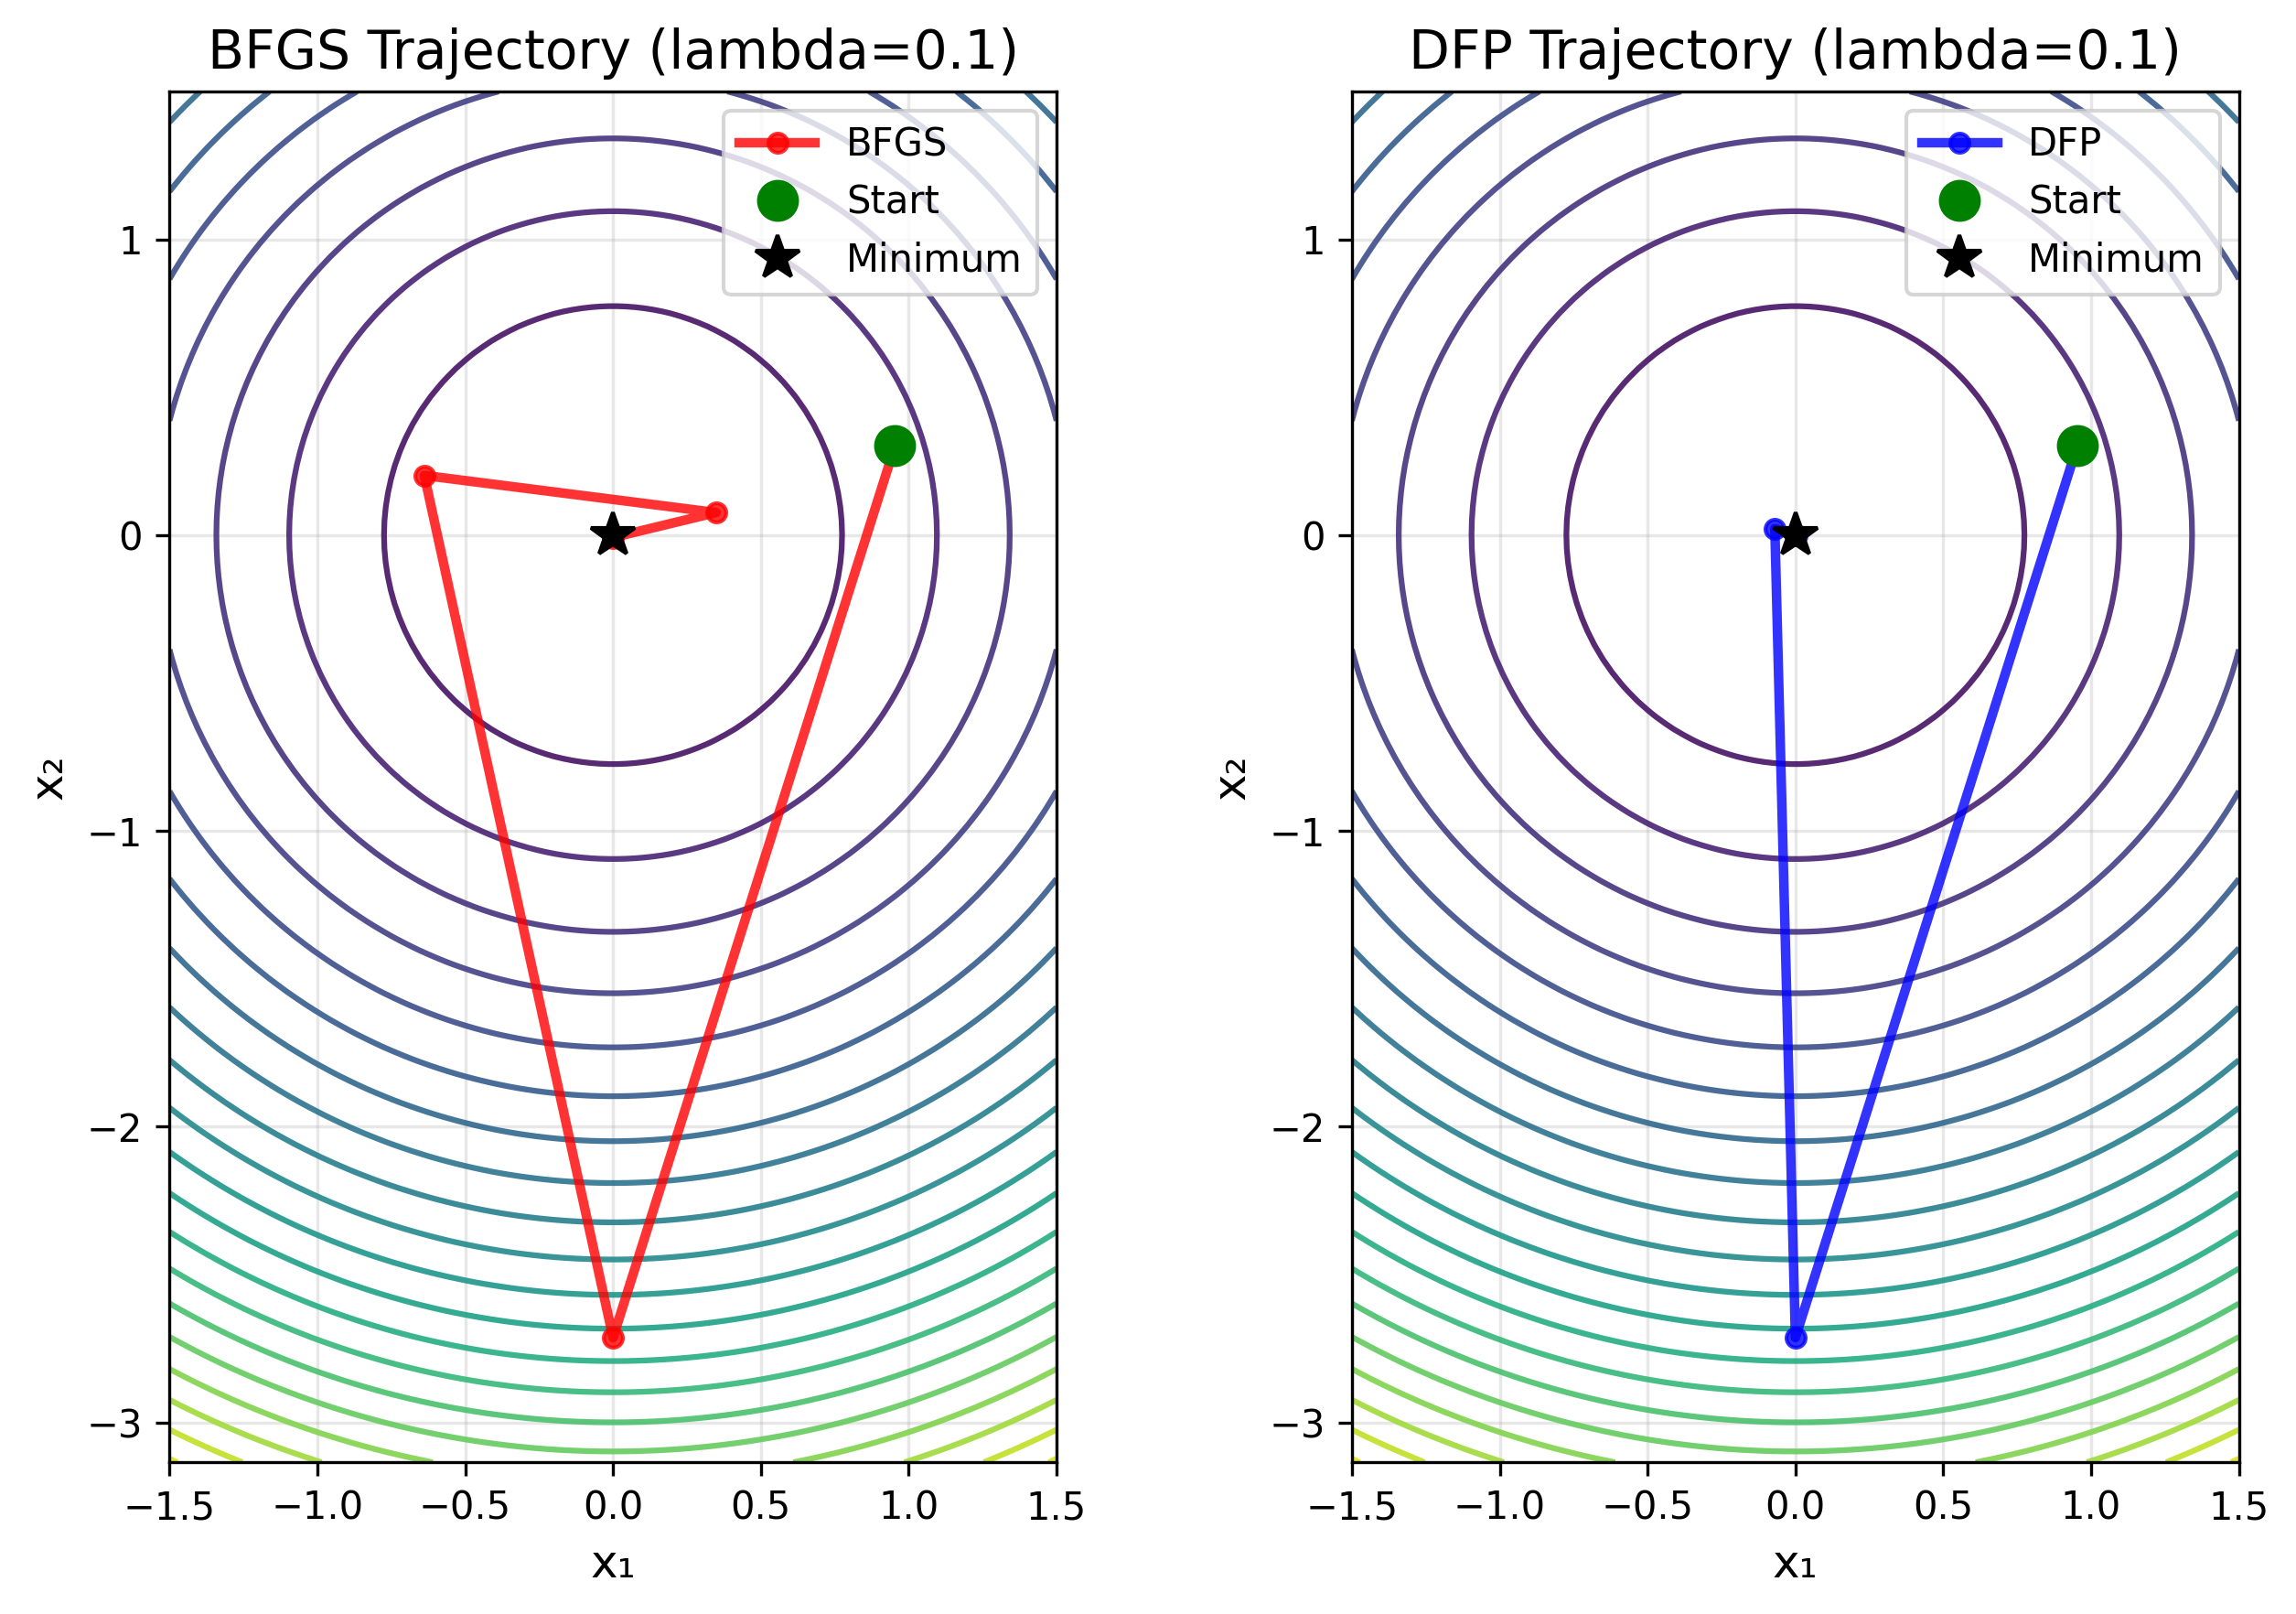
\includegraphics[width=\columnwidth]{../imgs/quasi_newton/bfgs_vs_dfp_0.1.png}
    \caption{BFGS と DFP の比較：$\lambda_1 = 0.1$}
    \label{fig:bfgs_vs_dfp_01}
\end{figure}

\begin{table}[h]
    \centering
    \begin{tabular}{|c|c|c|}
        \hline
        $\lambda_1$ & BFGS & DFP  \\
        \hline
        0.001       & 4    & 3    \\
        0.01        & 5    & 3    \\
        0.1         & 6    & 4    \\
        1           & 1    & 1    \\
        10          & 8    & 16   \\
        100         & 10   & 107  \\
        1000        & 12   & 1006 \\
        10000       & 15   & 9987 \\
        \hline
    \end{tabular}
    \caption{Convergence comparison between BFGS and DFP methods}
    \label{tab:bfgs_dfp_comparison}
\end{table}

\Cref{tab:bfgs_dfp_comparison}は、論文のtable1,2の内容を部分的に再現している。
数式による理論的な収束性の説明はここでは行わないが、この数値実験結果が本論文の要点であり、DFP法の方がBFGS法よりも著しく収束が遅いことを示している。

ところで、BFGSとDFPはかなり対称性が高い手法だが、このような非対称性はなぜ生じるのだろうか?

ここは論文にあった説明ではなく、単なる独自解釈も含まれるが、
本質的には「誤って大きく更新される($B_k$の固有値が小さすぎる)」ことよりも、「誤って小さくしか更新されない($B_k$の固有値が大きすぎる)」ことの方が、より深刻な事態を招きやすいという非対称性から生じているものと考えられる。

実際、\cref{tab:bfgs_dfp_comparison}の結果には、論文では実施されていない、$\lambda_1<1$の場合の結果も含めているが、この場合はわずかだがBFGS法の方が収束が遅い。この傾向の逆転自体は、BFGSとDFPの対称性から予想されるものである。
しかし、$\lambda_1<1$の場合は、固有値が小さすぎる、つまり、「誤って大きく更新される」ことになるので、$B_k$の修正がより簡単になっているので、その影響は極めて小さい。
固有値が大きすぎて、誤って少ししか更新されない場合の方が、$B_k$の修正がより困難であり、その時に有利なのがBFGS法である、という解釈は、BFGS法とDFP法の挙動の非対称性に対する一つの理解を提供するだろう。

\subsection{ Limited Memory BFGS (L-BFGS) }

Limited Memory Quasi-Newton法は、Quasi-Newton法を更に大規模最適化問題に特化させたものである。通常のQuasi-Newton法では、近似ヘッセ行列 $B_k$ を密行列として保存・更新するため、次元数 $n$ に対して $\order{n^2}$ の空間計算量を要する。

BFGS更新を用いたL-BFGS法 \citep{liuLimitedMemoryBFGS1989a}では、$B_k$ の情報を直接保存する代わりに、直近 $m$ 回分のベクトルペア $\{(s_i,y_i)\}_{i=k-m}^{k-1}$ のみを保存する(煩雑さを避ける都合上、本稿の各所で $k > m$ を暗黙裡に仮定しているが、それ以外の場合も同様に定義される)。 これにより、空間計算量は $\order{nm}$ となり、$m$ が十分小さい定数(10以下程度)の時はBFGS法の $\order{n^2}$ と比べて大幅に削減される。

\subsubsection{Compact Representation}

For convenience, define
\begin{equation}
    U_k = I - \rho_k y_k s_k^\top, \qquad
    V_k = I - \rho_k s_k y_k^\top.
\end{equation}
Then the BFGS updates can be written compactly as
\begin{align}
    B_{k+1} & = U_k B_k U_k^\top + \rho_k y_k y_k^\top, \label{eq:Bk_compact_lbfgs} \\
    H_{k+1} & = V_k H_k V_k^\top + \rho_k s_k s_k^\top. \label{eq:Hk_compact_lbfgs}
\end{align}

By recursively expanding $H_k$ over the most recent $m$ updates, one obtains
\begin{equation}
    H_k
    = V_{k-1} \cdots V_{k-m} H_k^{(0)} V_{k-m}^\top \cdots V_{k-1}^\top
    + \sum_{j=k-m}^{k-1} \bigg( \prod_{i=j+1}^{k-1} V_i \bigg)
    \rho_j s_j s_j^\top
    \bigg( \prod_{i=j+1}^{k-1} V_i \bigg)^\top,
\end{equation}
where $H_k^{(0)}$ denotes the initial approximation (often a scalar multiple of $I$).

\subsubsection{Two-Loop Recursion}

The above expansion can be applied to any vector $q$ without explicitly forming $H_k$.
Define $r = H_k q$.
Using the associative structure of matrix products, this can be computed using two short loops of length $m$,
leading to the celebrated \emph{two-loop recursion}.

\begin{algorithm}[htbp]
    \caption{Two-Loop Recursion for $r = H_k q$}
    \begin{algorithmic}[1]
        \STATE $q \gets \nabla f(x_k)$
        \FOR{$i = k-1, k-2, \dots, k-m$}
        \STATE $\alpha_i \gets \rho_i s_i^\top q$
        \STATE $q \gets q - \alpha_i y_i$
        \ENDFOR
        \STATE $r \gets H_k^{(0)} q$
        \FOR{$i = k-m, \dots, k-1$}
        \STATE $\beta \gets \rho_i y_i^\top r$
        \STATE $r \gets r + s_i (\alpha_i - \beta)$
        \ENDFOR
        \RETURN $r$
    \end{algorithmic}
\end{algorithm}

This algorithm requires $O(md)$ operations and $O(md)$ storage, where $d$ is the problem dimension.
No matrix inverses are formed explicitly.


\begin{proposition}
    Two-loop recursionの出力は、$r = H_k q$を満たす。
\end{proposition}
\begin{proof}
    このアルゴリズムが L-BFGS のコンパクト表現を正確に再現することを示す。

    まず次が成り立つ:
    \begin{equation*}
        V_i^\top q
        = (I - \rho_i s_i y_i^\top)^\top q
        = q - (\rho_i s_i^\top q) y_i.
    \end{equation*}
    したがって、最新のペアから最も古いペアへ向かってすべての \(V_i^\top\) を順に適用できる:
    \begin{equation*}
        \alpha_i = \rho_i s_i^\top q, \qquad
        q \gets q - \alpha_i y_i,
        \quad (i = k-1, k-2, \dots, k-m).
    \end{equation*}
    帰納法により、この後方ループを経た後のベクトルは次を満たす:
    \begin{equation*}
        q_{\mathrm{base}} =
        \qty(\prod_{t=k-m}^{k-1} V_t^\top) q_{\mathrm{orig}}.
    \end{equation*}
    したがって、この後方パスはすべての $V_i^\top$ を $q$ に適用すると同時に、
    対応するスカラー $\alpha_i$ を保存していることになる。

    後方パスの後、次を初期化する:
    $r = H_k^{(0)} q_{\mathrm{base}}$。
    その後、前方ループにおいて次の操作を行う:
    \begin{equation*}
        \beta_i = \rho_i y_i^\top r, \qquad
        r \gets r + s_i (\alpha_i - \beta_i),
        \quad (i = k-m, \dots, k-1),
    \end{equation*}
    これにより次が成り立つ:
    \begin{align*}
            & r+s_i (\alpha_i - \beta_i)                                                                                 \\
        ={} & r+ s_i \qty( \rho_i s_i^\top \qty(\prod_{t=i+1}^{k-1} V_t^\top) q_{\mathrm{orig}} - \rho_i y_i^\top r )    \\
        ={} & \qty(I - \rho_i s_i y_i^\top) r + \rho_i s_i s_i^\top \qty(\prod_{t=i+1}^{k-1} V_t^\top) q_{\mathrm{orig}} \\
        ={} & V_i r + \rho_i s_i s_i^\top \qty(\prod_{t=i+1}^{k-1} V_t^\top) q_{\mathrm{orig}}.
    \end{align*}
    したがって、任意の \(\ell \in [k-m, k]\) に対して次の不変式が帰納的に成り立つことを確認できる:
    \begin{equation*}
        r^{(\ell)} =
        \qty(\prod_{t=k-m}^{\ell-1} V_t)
        H_k^{(0)}
        \qty(\prod_{t=k-m}^{k-1} V_t^\top) q_{\mathrm{orig}}
        + \sum_{j=k-m}^{\ell-1}
        \qty(\prod_{i=j+1}^{\ell-1} V_i)
        \rho_j s_j s_j^\top
        \qty(\prod_{t=j+1}^{k-1} V_t^\top) q_{\mathrm{orig}}.
    \end{equation*}
    ゆえに、\(r^{(k)} = H_k q_{\mathrm{orig}}\) が成り立つ。
\end{proof}

以上より、2ループ再帰法は $H_k$ のコンパクト表現を正確に再現しつつ、行列を明示的に構成することを避けて計算出来ている。
この手法は $\order{md}$ の計算量と記憶量しか必要とせず、
数学的に厳密でありながら計算的にも高効率である。


\subsubsection{Initial Step Size}

$H_k^{0} = \gamma_k I$ where $\gamma_k = \frac{s_k^\top y_k}{\norm{y_k}^2}$
\cite{liuLimitedMemoryBFGS1989a,shannoMatrixConditioningNonlinear1978}

$\bar{G}_k=\int_0^1 \nabla^2 f(x_k + \tau \alpha_k p_k) \dd \tau$

$y_k = \bar{G}_k s_k$ より、

\begin{equation*}
    \frac{y_k^\top s_k}{\norm{y_k}^2} = \frac{(\bar{G}_k^{1/2} s_k)^\top (\bar{G}_k^{1/2} s_k)}{(\bar{G}_k^{1/2} s_k)^\top \bar{G}_k (\bar{G}_k^{1/2} s_k)}
\end{equation*}
より、これの逆数は $\bar{G}_k$ の固有値の一つの近似となる。
($\bar{G}_k^{1/2} s_k$ が固有ベクトルであれば、実際にこれの逆数はRayleigh商なので固有値になる。)

また、これはBB step size \cite{barzilaiTwoPointStepSize1988}のShort Step Sizeに相当する。

\subsection{line search}

\subsection*{具体例:三次関数と正則化手法の欠点}

ここでは具体例として
\[
    f(x)=x^2(x-1)=x^3-x^2
\]
を考える。勾配は
\[
    f'(x)=3x^2-2x = x(3x-2),
\]
よって臨界点は $x=0$(局所極大, $f''(0)=-2<0$) と $x=\frac{2}{3}$(局所極小, $f''(2/3)=2>0$) である。初期点を $x_0=\varepsilon>0$($\varepsilon$ は十分小さい正数) とし，探索方向を 1 次元かつ定数近似 $B_k\equiv M>0$ として
\[
    p_k=-B_k^{-1}f'(x_k)=-\frac{1}{M}f'(x_k)
\]
とする。初期点における方向は
\[
    p_0 = -\frac{1}{M}f'(\varepsilon) = -\frac{1}{M}\varepsilon(3\varepsilon-2)\approx \frac{2}{M}\varepsilon\qquad(\varepsilon\ll1).
\]

\paragraph{「越えるべき点」の定義}
ここでは直線探索で試行点が停留点 $x=\frac{2}{3}$ を下から超すことを到達基準とする(strong Wolfe の正当化に整合する考え方である) 。

\subsubsection*{強 Wolfe に基づく幾何的な倍々探索の内部反復数}
初期試行長を $\alpha_{\mathrm{init}}>0$ とし，試行長を倍々($\alpha\leftarrow2\alpha$) で増やしていく戦略を想定する。$p_0>0$ として，$x_0+\alpha p_0\ge 2/3$ となる最小の $\alpha^*$ は
\[
    \varepsilon + \alpha^* p_0 \ge \frac{2}{3}
    \quad\Longrightarrow\quad
    \alpha^* \ge \frac{\frac{2}{3}-\varepsilon}{p_0}
    \approx \frac{\frac{2}{3}}{(2\varepsilon/M)} = \frac{M}{3\varepsilon}\qquad(\varepsilon\ll1).
\]
倍々探索では $\alpha^*$ に到達するまでの試行回数 $t$ の下界は
\[
    t \ge \Big\lceil \log_2\!\Big(\frac{\alpha^*}{\alpha_{\mathrm{init}}}\Big)\Big\rceil
    \approx \log_2\!\Big(\frac{M}{3\varepsilon\,\alpha_{\mathrm{init}}}\Big).
\]
したがって $\varepsilon\to0^+$ に伴い，内部試行回数は対数的に発散する。

\subsubsection*{フルステップ更新でステップがノルムにより抑えられる場合}
フルステップ($\alpha=1$) を繰り返すモデルを考える。初期近傍では $f'(x)\approx -2x$ が成り立つため，
\[
    p(x)=-\frac{1}{M}f'(x)\approx \frac{2}{M}x.
\]
したがってフルステップ更新 $x_{k+1}=x_k+p(x_k)$ の漸近的な増分は
\[
    x_{k+1}\approx x_k\Big(1+\frac{2}{M}\Big),
\]
となり，$x_k$ は指数(幾何) 的に増加する。初期 $\varepsilon$ から $x_k$ が $\frac{2}{3}$ を超えるために必要な反復回数 $K$ は
\[
    \varepsilon\Big(1+\frac{2}{M}\Big)^K \ge \frac{2}{3}
    \quad\Longrightarrow\quad
    K \ge \frac{\ln\big(\frac{2}{3\varepsilon}\big)}{\ln\big(1+\frac{2}{M}\big)}.
\]
ここから分かるように，$M$ が大きい(ステップが小さい) と増加因子は 1 に近づき，$K$ は大きくなる。特に $\varepsilon$ が非常に小さい場合，$K$ は対数オーダーで大きくなり，実用的には到達が困難となる。

\paragraph{解釈と正則化手法の限界}
上の解析は，初期値が停留点 $x=0$ の非常に近くにある場合，探索方向が小さくなりすぎて停留点 $x=\frac{2}{3}$ を越えるのに多くの内部反復や外部反復を要することを示す。正則化($M$ を大きくする等) や保守的なステップ制限は数値安定性を与えるが，同時に必要な反復数を著しく増やす可能性がある。したがって設計上は，線探索の増加戦略や初期スケーリング($M$ の選択) ，あるいは適応的ステップ取扱いを組み合わせて，過度に小さい改善方向に固執しない工夫が必要である。

\section{Secant condition}

この時、新しい点 $x_{k+1}$ において再びヘッセ行列を近似するべく、$B_k$ を $B_{k+1}$ に更新する必要がある。近似行列$B_k$から、$s_k = x_{k+1} - x_k$ は探索ステップ、$y_k = \nabla f(x_{k+1}) - \nabla f(x_k)$ は勾配の変化量として、セカント条件 $B_{k+1} s_k = y_k$ を満たすように更新される。
セカント条件を課す理由は次のように正当化される。
まず $x_{k+1}$ 周りの二次近似モデルは次のように表される:
\begin{equation*}
    m_{k+1}(x) \defeq f(x_{k+1}) + \nabla f(x_{k+1})^\top (x - x_{k+1}) + \frac{1}{2} (x - x_{k+1})^\top B_{k+1} (x - x_{k+1}).
\end{equation*}
このモデルは、
\begin{gather*}
    m_{k+1}(x_{k+1}) = f(x_{k+1})\\
    \nabla m_{k+1}(x_{k+1}) = \nabla f(x_{k+1})
\end{gather*}
を満たす。そして、セカント条件を満たすならば、更に過去の点 $x_k$ においても
\begin{equation*}
    \nabla m_{k+1}(x_k) = \nabla f(x_{k+1}) - B_{k+1} s_k = \nabla f(x_{k})
\end{equation*}
を満たす為、セカント条件は勾配情報から妥当性のあるモデル関数を生成するための十分条件として正当化される。

もう一つの重要な概念が修正セカント条件である\citep{hassanModifiedSecantEquation2023}。その名の通り、セカント条件に修正を加え、修正後のベクトルペアによって近似ヘッセ行列を求め、最適化を行う。特にここでは関数値に基づく修正に注目する。従来のQuasi-Newton法では、関数値の情報は $B_k$ の更新には利用されてこなかったが、これを活用することで、より妥当性のある近似ヘッセ行列を得ることができる。

点 $x_{k+1}$ 周りでの二次近似 $m_{k+1}(x)$ は、そのヘッセ行列 $B_{k+1}$ によらずに、
\begin{equation}
    \begin{cases}
        m_{k+1}(x_{k+1}) = f(x_{k+1}) \\
        \nabla m_{k+1}(x_{k+1}) = \nabla f(x_{k+1})
    \end{cases} \label{eq:msec_xkp1}
\end{equation}
を常に満たす。
さらに、$B_{k+1}$ が通常のセカント条件を満たすならば、
\begin{equation}\label{eq:msec_gxk}
    \nabla m_{k+1}(x_k) = \nabla f(x_k)
\end{equation}
も満たすという点で正当化されていた。

これに対し、別の近似ヘッセ行列として $B^{\mathrm{Y}}_{k+1}$ を用いた
\begin{equation*}
    m_{k+1}^{\mathrm{Y}}(x) \defeq f(x_{k+1}) + \nabla f(x_{k+1})^\top (x - x_{k+1}) + \frac{1}{2} (x - x_{k+1})^\top B^{\mathrm{Y}}_{k+1} (x - x_{k+1})
\end{equation*}
では、\cref{eq:msec_xkp1}と同様の条件に加えて、
\begin{equation}\label{eq:msecY_fxk}
    m^{\mathrm{Y}}_{k+1}(x_k) = f(x_k)
\end{equation}
を満たすように更新式を定めることもできる。具体的には、
\begin{equation}\label{eq:msecY}
    B^{\mathrm{Y}}_{k+1}s_k = y_k + \frac{\max(0, 2(f_k- f_{k+1})+(g_{k+1}+g_k)^\top s_k)}{s_k^\top s_k} s_k
\end{equation}
という修正セカント条件を満たすと、部分的に\cref{eq:msecY_fxk}を満たせる。
(部分的と述べているのは、$\max(0, \cdot)$ の部分が0になる場合には\cref{eq:msecY_fxk}で等号が成立しないためである。この措置は $B^\mathrm{Y}_{k+1}$ の正定値性を保証するために導入されている。
% todo: \orange{todo: 裏付け}
)

また、近似の自由度を増やし、近似ヘッセ行列 $B_k^{\mathrm{Z}}$ とある定数 $c\in \bbR$ を用いて
\begin{equation*}
    m^\mathrm{Z}_{k+1}(x) \defeq f(x_{k+1}) + \nabla f(x_{k+1})^\top (x - x_{k+1}) + \frac{1}{2} (x - x_{k+1})^\top B_{k+1}^{\mathrm{Z}} (x - x_{k+1}) + c \norm{x-x_{k+1}}^3
\end{equation*}
とモデル関数を定めると、\cref{eq:msec_xkp1}と同様の条件に加えて、
\begin{equation}
    \begin{dcases}
        m^\mathrm{Z}_{k+1}(x_k) = f(x_k) \\
        \nabla m^\mathrm{Z}_{k+1}(x_k) = \nabla f(x_k)
    \end{dcases} \label{eq:msecZ_xk}
\end{equation}
の両方を満たすように $B^{\mathrm{Z}}_{k+1}$ と $c$ を取ることができる。
その十分条件の一つが
\begin{equation*}
    B^\mathrm{Z}_{k+1}s_k = y_k + \frac{6(f(x_k)-f(x_{k+1})) + 3 s_k^\top (\nabla f(x_k)+\nabla f(x_{k+1}))}{\norm{s_k}^2} s_k
\end{equation*}
という修正セカント条件である。

\subsection{Details of Derivation}

修正セカント条件による直線探索を用いた準Newton法について説明する。
本節では, Yuan による修正セカント条件を紹介する。
修正セカント条件は、$\{(s_i,y_i)\}_{i=k-m}^{k-1}$ のペアから近似ヘッセ行列 $B_{m,k}$ を求める際に、このペアをそのまま用いるのではなく、例えば $\{(s_i,y_i+\tau_i s_i)\}_{i=k-m}^{k-1}$ のように修正を加えたベクトルペアを用いることで、近似ヘッセ行列の精度を向上させる手法である。ここで、この修正分である $\tau_i$ は、各ペアごとに異なる値を取ることができ、Regularized Quasi-Newton法との違いが認められる。これはある意味で異方的な正則化と考えられる。

これらの本質は、通常のモデル関数が満たすべき性質である\cref{eq:msec_gxk}の代わりに、関数値の情報を基にした別の条件をモデル関数に課すことである。
更新後の行列が新しく課された条件を満たすための十分条件として、修正セカント条件は導出できる。
ここではそれらの導出を具体的にみると共に、不定値性を許容すれば従来手法を拡張できることも議論する。

\subsubsection{Yuan}

\cref{eq:msecY_fxk}の要請より、
\begin{equation*}
    m^\mathrm{Y}_{k+1}(x_k) = f(x_k)
    \iff f(x_{k+1}) - \nabla f(x_{k+1})^\top s_k + \frac12 s_k^\top B^\mathrm{Y}_{k+1} s_k = f(x_k)
\end{equation*}
が得られる。つまり、
\begin{equation*}
    f(x_k) - f(x_{k+1}) + \nabla f(x_{k+1})^\top s_k = \frac12 s_k^\top B^\mathrm{Y}_{k+1} s_k
\end{equation*}
である。特に、ある $C\in \bbR$ を用いて $B^\mathrm{Y}_{k+1} s_k = y_k - C s_k$ という形を仮定して代入すると、
\begin{align*}
     & f(x_k) - f(x_{k+1}) + \nabla f(x_{k+1})^\top s_k = \frac12 s_k^\top y_k - \frac{C}{2} \norm{s_k}^2 \\
     & \iff 2(f(x_k) - f(x_{k+1})) + (2\nabla f(x_{k+1})-y_k)^\top s_k = - C \norm{s_k}^2                 \\
     & \iff \frac{2(f(x_{k+1}) - f(x_k)) - (\nabla f(x_{k+1})+\nabla f(x_k))^\top s_k}{\norm{s_k}^2} = C
\end{align*}
を得られる。以上より、
\begin{equation*}
    B^\mathrm{Y}_{k+1} s_k = y_k - \frac{2(f(x_{k+1}) - f(x_k)) - (\nabla f(x_{k+1})+\nabla f(x_k))^\top s_k}{\norm{s_k}^2} s_k
\end{equation*}
という修正セカント条件を満たせば、\cref{eq:msecY_fxk}を満たすことが分かる。

そして、上記の修正セカント条件でも述べた通り、$B^\mathrm{Y}_{k+1} \succ 0$ を保証するため、分子において $\max(0, \cdot)$ を取ると、実際にYuanの提案した修正セカント条件となる。

\subsubsection{Zhang}
\label{subsubsec:zhang}

\cref{eq:msecZ_xk}の要請より、
\begin{align*}
    m^\mathrm{Z}_{k+1}(x_k) = f(x_k)
     & \iff f(x_{k+1})- \nabla f(x_{k+1})^\top s_k + \frac12 s_k^\top B^\mathrm{Z}_{k+1} s_k + c\norm{s_k}^3 = f(x_k) \\
    \nabla m^\mathrm{Z}_{k+1}(x_k) = \nabla f(x_k)
     & \iff \nabla f(x_{k+1})- B^\mathrm{Z}_{k+1} s_k - 3c\norm{s_k} s_k = \nabla f(x_k)
\end{align*}
が得られる、つまり、
\begin{align*}
    f(x_k) - f(x_{k+1})+ \nabla f(x_{k+1})^\top s_k & = \frac12 s_k^\top B^\mathrm{Z}_{k+1} s_k + c \norm{s_k}^3 \\
    s_k^\top (\nabla f(x_{k+1})-\nabla f(x_k))      & = s_k^\top B^\mathrm{Z}_{k+1} s_k + 3c \norm{s_k}^3
\end{align*}
であるので、この連立方程式を解くと、
\begin{align*}
    2(f(x_k)-f(x_{k+1})+\nabla f(x_{k+1})^\top s_k) - s_k^\top (\nabla f(x_{k+1})-\nabla f(x_k))                            & = -c \norm{s_k}^3    \\
    \frac{6(f(x_k)-f(x_{k+1})+\nabla f(x_{k+1})^\top s_k) - 3 s_k^\top (\nabla f(x_{k+1})-\nabla f(x_k))}{\norm{s_k}^2} s_k & = -3c \norm{s_k} s_k \\
    \frac{6(f(x_k)-f(x_{k+1})) + 3 s_k^\top (\nabla f(x_{k+1})+\nabla f(x_k))}{\norm{s_k}^2} s_k                            & = -3c \norm{s_k} s_k
\end{align*}
を得られる。以上より、$\nabla^2 m^\mathrm{Z}_{k+1}(x_{k+1}) = B^\mathrm{Z}_{k+1}$ は
\begin{equation*}
    B^\mathrm{Z}_{k+1}s_k = y_k + \frac{6(f(x_k)-f(x_{k+1})) + 3 s_k^\top (\nabla f(x_k)+\nabla f(x_{k+1}))}{\norm{s_k}^2} s_k
\end{equation*}
という修正セカント条件を満たせば、\cref{eq:msecZ_xk}を満たすことが分かる。

\subsection{Clipping}

以上2つの修正セカント条件を組み合わせることも可能である。

上記はいずれも $B_{k+1} s_k = y_k + \tau_k s_k$ という形をしている。そこで、\cref{subsubsec:zhang}の修正セカント条件における $\tau_k$ の部分を、\cref{subsubsec:zhang}の修正セカント条件における $\tau_k$ を中心として一定の範囲内に収めるようにクリッピングすると、極端に3次導関数の寄与が大きくなることを防ぐことができる。

\subsection{Other Secant-like Equation}

\Cref{subsubsec:zhang}条件は、別の十分条件が存在し、それを導出することが出来る。詳細は省略するが、結果のみ以下に示す。

\begin{equation*}
    B^\mathrm{O}_{k+1} s_k = \qty(6\frac{f(x_k) - f(x_{k+1}) + \nabla f(x_{k+1})^\top s_k}{s_k^\top y_k}-2) y_k
\end{equation*}

\subsection{other storing}

For storing the curvature information, there are several topics.\\

\textbf{agg-BFGS} \citep{berahasLimitedmemoryBFGSDisplacement2022}: Instead of discarding the oldest and adding the newest, we can aggregate the information.\\

\textbf{multi-secant} \citep{leeAdvancingMultiSecantQuasiNewton2025}:\\
\quad Standard:
\begin{equation*}
    \quad s_i = x_{i+1} - x_i, \quad y_i = \nabla f(x_{i+1}) - \nabla f(x_i), \quad (i = k-m, \ldots, k)
\end{equation*}
\quad Anchored at most recent:
\begin{equation*}
    \quad s_i = x_{k+1} - x_i, \quad y_i = \nabla f(x_{k+1}) - \nabla f(x_i), \quad (i = k-m, \ldots, k)
\end{equation*}


\section{Positive Definiteness of Hessian Approximation}

そもそもBFGS更新自体が、正定値性を仮定した上で成り立っている。

\subsection{How to make Positive Definite}

定性的な性質として、
$B_k + \mu_k I$は正定値であってほしいが、その最小固有値は可能な限り小さくあってほしい。
例えば、ある定数$\mu_{\min}>0$が存在して、
$B_k + \mu_k I \succeq \mu_{\min} I$が成り立つとすると、
$\norm{d_k} = \norm{-(B_k + \mu I)^{-1} \nabla f(x_k)} \leq \frac{1}{\mu_{\min}} \norm{\nabla f(x_k)}$が成り立ってしまい、常に$x_{k+1}\gets x_k + d_k$と更新されたとしても、$\norm{x^* - x_k}$が十分小さい場合には、十分な減少が得られない可能性がある。

1. cautious update

単純に飛ばす。非凸性が激しい場合に、必ずしも好ましくない。

2. kanzow +$\mu_k$ I

最小限のregularizationで済む可能性が高い。
ただし、正定値性が必ずしも保証されるとは限らず、
それゆえに、鞍点に陥る可能性が残されている。

3. modified secant

いわゆるmodified secantとして、最も安易な方法。
$\mu$が大きすぎて、

4. 真の$\lambda_{\min}$を計算する。

L-BFGSであると、HVPが軽いので、比較的高速に求まるが、
定数倍はそれなりにかかる。

5. damped BFGS

まともそう
\href{https://arxiv.org/pdf/2012.05783}{arxiv}


$\mu_k$がいくらかあると、ずれるみたいなことをいいたい。
BFGSの時は、どのくらい誤差に差が出るか、それがどのくらい失われるのか。


\begin{assumption}
    以下の仮定を置く。
    \begin{enumerate}
        \item \(H\in\bbR^{n\times n}\) は対称正定(すなわち \(H=H^\top\) かつ \(x^\top H x>0\) for all \(x\neq0\))。
        \item \(s,y\in\bbR^n\) は非零ベクトルで、内積 \(s_k^\top y>0\) を満たす(ただし後に \(s_k^\top y\to0^+\) を考える)。
        \item 更新係数を \(\displaystyle \rho=\frac{1}{s_k^\top y}\) と定め、逆BFGS の逆ヘッセ近似の更新を
              \[
                  H_{+} \;=\; (I-\rho s_k y_k^\top)\,H\,(I-\rho y_k s_k^\top) \;+\; \rho\, s_k s_k^\top
              \]
              とする。
    \end{enumerate}
\end{assumption}

\begin{theorem}
    上の仮定の下で、\(s_k^\top y_k \to 0^+\)(すなわち \(\rho\to +\infty\))の極限において、
    \[
        \lambda_{\max}(H_{+}) \to +\infty.
    \]
    さらに発散速度は二乗的であり、正確には
    \[
        \lambda_{\max}(H_{+}) = \Omega\!\qty(\frac{1}{(s_k^\top y)^2})
    \]
    が成立する(係数は \(\|s\|^2\, (y_k^\top H y)\) に比例する)。
\end{theorem}

\begin{proof}
    最大固有値はレイリー商の最大値として定義される。ここではレイリー商を単位ベクトルに限定して扱う。すなわち
    \[
        \lambda_{\max}(H_{+}) = \max_{\|v\|=1} v^\top H_{+} v.
    \]
    従って任意の単位ベクトル \(v\) に対して成り立つ下界を与えれば、それは最大固有値の下界となる。特に自然な候補 \(v=\dfrac{s}{\|s\|}\) を取る(\(s\neq0\) を仮定している)ことで下界を得る。

    まず一般の単位ベクトル \(v\) に関して、更新式から直接に次が成り立つ(展開せずの等式):
    \[
        \begin{aligned}
            v^\top H_{+} v
             & = v^\top \qty((I-\rho s_k y_k^\top) H (I-\rho y_k s_k^\top)) v + \rho (s_k^\top v)^2        \\
             & = \qty((I-\rho y_k s_k^\top) v)^\top H \qty((I-\rho y_k s_k^\top) v) + \rho (s_k^\top v)^2.
        \end{aligned}
    \]
    ここで右辺は非負かつ \(H\) の正定性により下に抑えられないことに注意する。

    今 \(v=\dfrac{s}{\|s\|}\) を代入する。まず
    \[
        \|v\|=1,\qquad s_k^\top v = \|s\|.
    \]
    また
    \[
        (I-\rho y_k s_k^\top)\,v = v - \rho y_k (s_k^\top v) = \frac{s}{\|s\|} - \rho y_k \|s\|
        = \frac{1}{\|s\|}\,s_k - \rho \|s\|\, y.
    \]
    これを \(w\) と定義する:
    \[
        w  \defeq  (I-\rho y_k s_k^\top)\,v = \frac{s}{\|s\|} - \rho \|s\|\, y.
    \]
    すると
    \[
        \begin{aligned}
            v^\top H_{+} v
             & = w^\top H w + \rho (s_k^\top v)^2 \\
             & = w^\top H w + \rho \|s\|^2.
        \end{aligned}
    \]

    次に \(w^\top H w\) を展開して主要な \(\rho\) 依存性を明示する。計算を丁寧に行うと(スカラーの結合法則に注意)、
    \[
        \begin{aligned}
            w          & = \frac{s}{\|s\|} - \rho \|s\|\, y,         \\
            w^\top H w & = \qty(\frac{s}{\|s\|} - \rho \|s\| y)^\top
            H \qty(\frac{s}{\|s\|} - \rho \|s\| y)                   \\
                       & = \frac{1}{\|s\|^2}\, s_k^\top H s
            -2\rho\, (y_k^\top H s)
            + \rho^2 \|s\|^2 (y_k^\top H y).
        \end{aligned}
    \]
    したがって
    \[
        \begin{aligned}
            v^\top H_{+} v
             & = \frac{1}{\|s\|^2}\, s_k^\top H s
            -2\rho\, (y_k^\top H s)
            + \rho^2 \|s\|^2 (y_k^\top H y)
            + \rho \|s\|^2.
        \end{aligned}
    \]

    簡潔化のためにスカラー記号を導入して整理しておく:
    \begin{equation}\label{eq:scalar_notation}
        \alpha  \defeq  s_k^\top H s,\qquad \beta  \defeq  y_k^\top H s,\qquad \gamma  \defeq  y_k^\top H y,\qquad a \defeq \|s\|^2(>0).
    \end{equation}
    このとき
    \begin{equation}\label{eq:v_H_v_form}
        v^\top H_{+} v
        = \frac{\alpha}{a} - 2\rho \beta + \rho^2 a \gamma + \rho a.
    \end{equation}

    ここで \(\rho = 1/(s_k^\top y)\) を用いて、\(s_k^\top y\to 0^+\)(すなわち \(\rho\to+\infty\))の極限を考える。まず仮定から \(H\) は正定なので \(\gamma = y_k^\top H y>0\)(ただし \(y\neq0\))が成り立つ。したがって右辺の支配項は \(\rho^2 a \gamma\) である。より厳密に言えば、
    \[
        \rho^2 a \gamma - 2\rho \beta + \rho a + \frac{\alpha}{a}
        = \rho^2 a \gamma \qty( 1 - \frac{2\beta}{\rho a \gamma} + \frac{1}{\rho \gamma} + \frac{\alpha}{\rho^2 a^2 \gamma} ).
    \]
    項ごとに \(\rho\to\infty\) を取ると括弧内は 1 に収束するため、総体として
    \[
        v^\top H_{+} v \sim \rho^2 a \gamma
        = \frac{\|s\|^2\, (y_k^\top H y)}{(s_k^\top y)^2}
        \quad (\,s_k^\top y\to 0^+\,).
    \]

    したがって単位ベクトル \(v=\dfrac{s}{\|s\|}\) に対するレイリー商は \((s_k^\top y)^{-2}\) オーダーで発散する。最大固有値は単位ベクトル上の最大値なので(特に上で取った値は下界になる)
    \[
        \lambda_{\max}(H_{+}) \ge v^\top H_{+} v \sim \frac{\|s\|^2\, (y_k^\top H y)}{(s_k^\top y)^2} \to +\infty
        \quad(\,s_k^\top y\to 0^+\,).
    \]

    従って示すべき結論 \(\lambda_{\max}(H_{+})\to+\infty\) が得られる。発散速度の評価も上の漸近から明らかである。
\end{proof}

\paragraph{補足}
\begin{itemize}
    \item もし \(y_k^\top H y=0\) のような特殊ケースが成り立てば(通常の仮定の下では起こりえないが理論的には可能)、上で支配的だった \(\rho^2\) 項が消えるため発散速度は遅くなるか、キャンセルによって発散しない可能性がある。従って本証明は \(H\) の正定性および \(y\neq0\) を本質的に利用している。
    \item 本証明ではレイリー商を単位ベクトルに限定したので、提示された不等式(正規化を忘れた形)に対しても自然な修正として
          \[
              \lambda_{\max}(H_{+}) \;\ge\; \frac{\qty((I-\rho y_k s_k^\top)s)^\top H \qty((I-\rho y_k s_k^\top)s) + \rho \|s\|^4}{\|s\|^2}
          \]
          が成り立つことが分かる(右辺は \(v=\dfrac{s}{\|s\|}\) を代入した場合の値に一致する)。
\end{itemize}


\section{Regularization}

\begin{itemize}
    \item[\textbullet] Combination with Trust-Region {\footnotesize\citep{burdakovEfficientlyCombiningLimitedmemory2017}}
    \item[\textbullet] Regularized Proximal Quasi-Newton {\footnotesize\citep{kanzowEfficientRegularizedProximal2022a}}
          \begin{itemize}
              \item Proximal Operator is used.
          \end{itemize}
    \item[\textbullet] Cubic Regularization {\footnotesize\citep{kamzolovCubicRegularizationKey2023}}
          \begin{itemize}
              \item ``Cubic Regularized Quasi-Newton Methods'' is the same.
          \end{itemize}
    \item[\textbullet] Cubic Regularization (For non-smooth) {\footnotesize\citep{wangConvergenceRatesRegularized2025}}
          \begin{itemize}
              \item For theoretical analysis, the CRN seems to be more suitable.
          \end{itemize}
    \item[\textbullet] SR1+Cubic Regularization Newton {\footnotesize\citep{ranganathSymmetricRankOneQuasiNewton2025}}
          \begin{itemize}
              \item For deep learning. Maybe we can test our method similarly.
          \end{itemize}
\end{itemize}


\bibliographystyle{plain}
\bibliography{../L-BFGS}

\end{document}

